% Options for packages loaded elsewhere
\PassOptionsToPackage{unicode}{hyperref}
\PassOptionsToPackage{hyphens}{url}
%
\documentclass[
  man,floatsintext]{apa6}
\usepackage{amsmath,amssymb}
\usepackage{iftex}
\ifPDFTeX
  \usepackage[T1]{fontenc}
  \usepackage[utf8]{inputenc}
  \usepackage{textcomp} % provide euro and other symbols
\else % if luatex or xetex
  \usepackage{unicode-math} % this also loads fontspec
  \defaultfontfeatures{Scale=MatchLowercase}
  \defaultfontfeatures[\rmfamily]{Ligatures=TeX,Scale=1}
\fi
\usepackage{lmodern}
\ifPDFTeX\else
  % xetex/luatex font selection
\fi
% Use upquote if available, for straight quotes in verbatim environments
\IfFileExists{upquote.sty}{\usepackage{upquote}}{}
\IfFileExists{microtype.sty}{% use microtype if available
  \usepackage[]{microtype}
  \UseMicrotypeSet[protrusion]{basicmath} % disable protrusion for tt fonts
}{}
\makeatletter
\@ifundefined{KOMAClassName}{% if non-KOMA class
  \IfFileExists{parskip.sty}{%
    \usepackage{parskip}
  }{% else
    \setlength{\parindent}{0pt}
    \setlength{\parskip}{6pt plus 2pt minus 1pt}}
}{% if KOMA class
  \KOMAoptions{parskip=half}}
\makeatother
\usepackage{xcolor}
\usepackage{graphicx}
\makeatletter
\def\maxwidth{\ifdim\Gin@nat@width>\linewidth\linewidth\else\Gin@nat@width\fi}
\def\maxheight{\ifdim\Gin@nat@height>\textheight\textheight\else\Gin@nat@height\fi}
\makeatother
% Scale images if necessary, so that they will not overflow the page
% margins by default, and it is still possible to overwrite the defaults
% using explicit options in \includegraphics[width, height, ...]{}
\setkeys{Gin}{width=\maxwidth,height=\maxheight,keepaspectratio}
% Set default figure placement to htbp
\makeatletter
\def\fps@figure{htbp}
\makeatother
\setlength{\emergencystretch}{3em} % prevent overfull lines
\providecommand{\tightlist}{%
  \setlength{\itemsep}{0pt}\setlength{\parskip}{0pt}}
\setcounter{secnumdepth}{-\maxdimen} % remove section numbering
% Make \paragraph and \subparagraph free-standing
\ifx\paragraph\undefined\else
  \let\oldparagraph\paragraph
  \renewcommand{\paragraph}[1]{\oldparagraph{#1}\mbox{}}
\fi
\ifx\subparagraph\undefined\else
  \let\oldsubparagraph\subparagraph
  \renewcommand{\subparagraph}[1]{\oldsubparagraph{#1}\mbox{}}
\fi
\newlength{\cslhangindent}
\setlength{\cslhangindent}{1.5em}
\newlength{\csllabelwidth}
\setlength{\csllabelwidth}{3em}
\newlength{\cslentryspacingunit} % times entry-spacing
\setlength{\cslentryspacingunit}{\parskip}
\newenvironment{CSLReferences}[2] % #1 hanging-ident, #2 entry spacing
 {% don't indent paragraphs
  \setlength{\parindent}{0pt}
  % turn on hanging indent if param 1 is 1
  \ifodd #1
  \let\oldpar\par
  \def\par{\hangindent=\cslhangindent\oldpar}
  \fi
  % set entry spacing
  \setlength{\parskip}{#2\cslentryspacingunit}
 }%
 {}
\usepackage{calc}
\newcommand{\CSLBlock}[1]{#1\hfill\break}
\newcommand{\CSLLeftMargin}[1]{\parbox[t]{\csllabelwidth}{#1}}
\newcommand{\CSLRightInline}[1]{\parbox[t]{\linewidth - \csllabelwidth}{#1}\break}
\newcommand{\CSLIndent}[1]{\hspace{\cslhangindent}#1}
\ifLuaTeX
\usepackage[bidi=basic]{babel}
\else
\usepackage[bidi=default]{babel}
\fi
\babelprovide[main,import]{english}
% get rid of language-specific shorthands (see #6817):
\let\LanguageShortHands\languageshorthands
\def\languageshorthands#1{}
% Manuscript styling
\usepackage{upgreek}
\captionsetup{font=singlespacing,justification=justified}

% Table formatting
\usepackage{longtable}
\usepackage{lscape}
% \usepackage[counterclockwise]{rotating}   % Landscape page setup for large tables
\usepackage{multirow}		% Table styling
\usepackage{tabularx}		% Control Column width
\usepackage[flushleft]{threeparttable}	% Allows for three part tables with a specified notes section
\usepackage{threeparttablex}            % Lets threeparttable work with longtable

% Create new environments so endfloat can handle them
% \newenvironment{ltable}
%   {\begin{landscape}\centering\begin{threeparttable}}
%   {\end{threeparttable}\end{landscape}}
\newenvironment{lltable}{\begin{landscape}\centering\begin{ThreePartTable}}{\end{ThreePartTable}\end{landscape}}

% Enables adjusting longtable caption width to table width
% Solution found at http://golatex.de/longtable-mit-caption-so-breit-wie-die-tabelle-t15767.html
\makeatletter
\newcommand\LastLTentrywidth{1em}
\newlength\longtablewidth
\setlength{\longtablewidth}{1in}
\newcommand{\getlongtablewidth}{\begingroup \ifcsname LT@\roman{LT@tables}\endcsname \global\longtablewidth=0pt \renewcommand{\LT@entry}[2]{\global\advance\longtablewidth by ##2\relax\gdef\LastLTentrywidth{##2}}\@nameuse{LT@\roman{LT@tables}} \fi \endgroup}

% \setlength{\parindent}{0.5in}
% \setlength{\parskip}{0pt plus 0pt minus 0pt}

% Overwrite redefinition of paragraph and subparagraph by the default LaTeX template
% See https://github.com/crsh/papaja/issues/292
\makeatletter
\renewcommand{\paragraph}{\@startsection{paragraph}{4}{\parindent}%
  {0\baselineskip \@plus 0.2ex \@minus 0.2ex}%
  {-1em}%
  {\normalfont\normalsize\bfseries\itshape\typesectitle}}

\renewcommand{\subparagraph}[1]{\@startsection{subparagraph}{5}{1em}%
  {0\baselineskip \@plus 0.2ex \@minus 0.2ex}%
  {-\z@\relax}%
  {\normalfont\normalsize\itshape\hspace{\parindent}{#1}\textit{\addperi}}{\relax}}
\makeatother

% \usepackage{etoolbox}
\makeatletter
\patchcmd{\HyOrg@maketitle}
  {\section{\normalfont\normalsize\abstractname}}
  {\section*{\normalfont\normalsize\abstractname}}
  {}{\typeout{Failed to patch abstract.}}
\patchcmd{\HyOrg@maketitle}
  {\section{\protect\normalfont{\@title}}}
  {\section*{\protect\normalfont{\@title}}}
  {}{\typeout{Failed to patch title.}}
\makeatother

\usepackage{xpatch}
\makeatletter
\xapptocmd\appendix
  {\xapptocmd\section
    {\addcontentsline{toc}{section}{\appendixname\ifoneappendix\else~\theappendix\fi\\: #1}}
    {}{\InnerPatchFailed}%
  }
{}{\PatchFailed}
\keywords{cooperation, behavioural economics, political views, Social Dominance Orientation, income redistribution, longitudinal}
\usepackage{lineno}

\linenumbers
\usepackage{csquotes}
\raggedbottom
\usepackage{setspace}
\AtBeginEnvironment{tabular}{\singlespacing}
\AtBeginEnvironment{lltable}{\singlespacing}
\AtBeginEnvironment{tablenotes}{\doublespacing}
\captionsetup[table]{font={stretch=1.5}}
\captionsetup[figure]{font={stretch=1.5}}
\nolinenumbers
\note{\raggedright * Correspondence concerning this article should be addressed to Scott Claessens, Level 2, Building 302, 23 Symonds Street, Auckland, New Zealand. \text{E-mail:} \href{scott.claessens@gmail.com}{\nolinkurl{scott.claessens@gmail.com}} \par Word count = 4984 words \par Author \text{biographies:} \begin{itemize} \item \textbf{Scott Claessens} is a Research Fellow in the School of Psychology at the University of Auckland. He is interested in the evolution of cooperation, culture, and political ideology. \item \textbf{Chris G Sibley} is a Professor in the School of Psychology at the University of Auckland. He is the Principal Investigator for the New Zealand Attitudes and Values Study. \item \textbf{Ananish Chaudhuri} is a Professor of Experimental Economics in the Department of Economics at the University of Auckland. He has a broad research agenda in behavioural economics, including a significant amount of cross-disciplinary work. \item \textbf{Quentin D Atkinson} is a Professor in the School of Psychology at the University of Auckland and co-Director of the University of Auckland Behavioural Insights Exchange (UoABIX). He is interested in the origins of linguistic diversity, the function of religion, the psychology of climate change, and how evolved cognitive biases shape our social behaviour. \end{itemize}}
\ifLuaTeX
  \usepackage{selnolig}  % disable illegal ligatures
\fi
\IfFileExists{bookmark.sty}{\usepackage{bookmark}}{\usepackage{hyperref}}
\IfFileExists{xurl.sty}{\usepackage{xurl}}{} % add URL line breaks if available
\urlstyle{same}
\hypersetup{
  pdftitle={Cooperative phenotype predicts political views on hierarchy and redistribution eighteen months later},
  pdfauthor={Scott Claessens1*, Chris G Sibley1, Ananish Chaudhuri2,3, \& Quentin D Atkinson1,4},
  pdflang={en-EN},
  pdfkeywords={cooperation, behavioural economics, political views, Social Dominance Orientation, income redistribution, longitudinal},
  hidelinks,
  pdfcreator={LaTeX via pandoc}}

\title{Cooperative phenotype predicts political views on hierarchy and redistribution eighteen months later}
\author{Scott Claessens\textsuperscript{1*}, Chris G Sibley\textsuperscript{1}, Ananish Chaudhuri\textsuperscript{2,3}, \& Quentin D Atkinson\textsuperscript{1,4}}
\date{}


\shorttitle{Cooperation politics longitudinal}

\affiliation{\vspace{0.5cm}\textsuperscript{1} \footnotesize School of Psychology, University of Auckland, Auckland, New Zealand\\\textsuperscript{2} \footnotesize Department of Economics, University of Auckland, Auckland, New Zealand\\\textsuperscript{3} \footnotesize CESifo, Munich, Germany\\\textsuperscript{4} \footnotesize Max Planck Institute for the Science of Human History, Jena, Germany}

\abstract{%
Cross-sectional research has identified robust correlations between cooperative behaviour in economic games and political views, but this research is limited in its ability to draw causal inferences. Here, we conducted a longitudinal cross-lagged panel study of cooperation and political views with a New Zealand sample (n = 631). Across two waves separated by eighteen months, we measured self-reported political views and employed a battery of economic games to estimate people's general preferences for cooperation. We found that this ``cooperative phenotype'' predicted future variation in some of our measures of political views, including Social Dominance Orientation and support for income redistribution. Income attribution beliefs and political party support were not related to the cooperative phenotype over time. None of these variables predicted future variation in the cooperative phenotype. These results suggest that cooperative predispositions may play a causal role in the expression of certain political views.
}



\begin{document}
\maketitle

\nolinenumbers

\hypertarget{introduction}{%
\section{Introduction}\label{introduction}}

People vary in their political voting patterns, policy views, and party
support. In part, this variation is thought to be due to individual differences
in political ideology, defined as ``a set of stable, interrelated beliefs and
attitudes that organise views on political and social issues'' (Jost, Federico, \& Napier, 2009).

It has long been assumed that one's ideology is primarily acquired through
partisanship that is learned from one's parents and peers or soaked up through
mass media (Campbell, Converse, Miller, \& Stokes, 1960; Zaller, 1992). This assumption continues today, with
researchers arguing that differing political views are due mainly to partisan
divides rather than any enduring psychological or dispositional differences
(Brandt, Reyna, Chambers, Crawford, \& Wetherell, 2014). However, this claim is at odds with research highlighting the
importance of dispositional variables in the expression of political ideology.
This body of work has revealed that, compared to liberals, conservatives tend to
be more sensitive to threats and uncertainty (Jost, Glaser, Kruglanski, \& Sulloway, 2003) and express a greater
need for closure (Jost et al., 2003). Different variables have also been linked to
different measures of political ideology. Social conservatives and people higher
in Right Wing Authoritarianism (RWA; an ideological measure of norm-adherence
and group conformity) (Altemeyer, 1981) tend to be more sensitive to disgusting
stimuli (Inbar, Pizarro, Iyer, \& Haidt, 2012), while economic conservatives and people higher in Social
Dominance Orientation (SDO; an ideological measure of support for hierarchy and
dominance) (Pratto, Sidanius, Stallworth, \& Malle, 1994) tend to exhibit higher levels of physical dominance and
formidability (Petersen \& Laustsen, 2019).

Prosocial preferences have also been shown to vary across the ideological
landscape. Research has found a negative relationship between SDO and
Social Value Orientation (SVO), a self-reported measure of prosocial preferences
in which people make hypothetical allocations of money between themselves and
others (Chirumbolo, Leone, \& Desimoni, 2016; Haesevoets, Reinders Folmer, \& Van Hiel, 2015). Research has also revealed robust
correlations between political views and cooperative behaviour in economic
games. Economic games (\emph{i.e.}, social decision-making tasks that involve real
money) are tools that elicit prosocial preferences while avoiding the
desirability issues that plague self-report methods (Pisor, Gervais, Purzycki, \& Ross, 2020). Studies using
economic games have shown that people higher in SDO tend to share less money in
social dilemma games that pit self-interest against collective-interest
(Haesevoets, Reinders Folmer, Bostyn, \& Van Hiel, 2018; Haesevoets et al., 2015; Halali, Dorfman, Jun, \& Halevy, 2018). A recent meta-analysis of data
from over 3,000 participants found a reliable negative correlation between SDO
and cooperative behaviour in economic games, albeit with a small effect size
(Thielmann, Spadaro, \& Balliet, 2020).

Extending this work, Claessens, Sibley, Chaudhuri, and Atkinson (2023) found that SDO was negatively correlated
with a ``cooperative phenotype'' latent variable, a general behavioural
disposition for cooperation that is uncovered via a battery of economic games
(Peysakhovich, Nowak, \& Rand, 2014). Conceptually similar to SVO but measured across a variety
of incentivised contexts, the cooperative phenotype reflects an unconditional
concern for the welfare of others when there is a possibility for exploitation
(Thielmann, Hilbig, \& Zettler, 2022). This common factor underlying prosocial behaviour in economic
games has been replicated across a wide variety of samples and cultures
(Chierchia, Lesemann, Snower, Vogel, \& Singer, 2017; Claessens et al., 2023; Peysakhovich et al., 2014; Reigstad, Strømland, \& Tinghög, 2017; Yamagishi et al., 2013).

The correlation between political views and the cooperative phenotype provides
further evidence for a dispositional basis for political ideology. However, this
correlation raises the question of whether and how these variables causally
influence one another. At least three causal models are compatible with a
cross-sectional correlation between political views and the cooperative
phenotype.

Prior work has tended to adopt a \emph{cooperation-as-outcome} model. Under this
model, biological and environmental factors interact to produce political
views (Duckitt \& Sibley, 2009) and people's political views then influence how they
behave in economic games. This causal model is often assumed \emph{a priori} to
explain cross-sectional correlations between politics and behaviour in economic
games. For example, Grünhage and Reuter (2020) write that ``political orientation
\emph{predisposes for} a more trusting or cooperative behavior'' (italics added; p.~22).

Alternatively, under the \emph{cooperation-as-antecedent} model, biological and
environmental factors interact to produce the behavioural predispositions
captured by economic games, and these behavioural predispositions influence the
expression of particular political views. This causal model is predicted by the
dual evolutionary framework of political ideology (Claessens, Fischer, Chaudhuri, Sibley, \& Atkinson, 2020), which
explains political attitudes as shaped in part by basic social drives that were
favoured during human evolution. Human group living evolved via two key shifts
(Tomasello, Melis, Tennie, Wyman, \& Herrmann, 2012); a shift towards increased cooperation with others, and a shift
towards conformity to and enforcement of group-wide social norms. According to
the dual evolutionary framework, variation in general drives for cooperation and
group conformity arises from the interaction between heritable individual
differences and socio-ecological environments. These general drives for
cooperation and group conformity, together with individuals' immediate social
context, produce variation in two dimensions of political ideology, often
referred to as economic and social ideology (Claessens et al., 2020). This causal
pathway --- from behavioural predispositions to politics --- is captured by
Van Lange, Bekkers, Chirumbolo, and Leone (2012), who write that ``political preferences and voting are \emph{partially
rooted in} interpersonal orientations'' (italics added; p.~469).

Finally, the \emph{common-cause} model predicts that both behaviour and political
views are caused by the same biological and environmental factors, but do not
directly influence one another over time. This model is inspired by recent
longitudinal evidence showing that personality does not causally precede
political ideology, but instead personality and political ideology develop
together in parallel, likely due to common causes from biological and
environmental factors (Osborne \& Sibley, 2020). Similarly, the common-cause model predicts
that political ideology and the cooperative phenotype will be correlated, not
because they influence one another over time, but because they share the same
biological and environmental causes. This model is also consistent with the dual
evolutionary framework of political ideology, insofar as heritable individual
differences and socio-ecological environments influence both cooperative
behaviour and political ideology simultaneously.

Figure \ref{fig:theoreticalModels} provides an overview of these causal
models. All three models predict a cross-sectional correlation between political
ideology and cooperative behaviour. As such, previous cross-sectional work
cannot distinguish between them. Previous longitudinal work has shown that
cooperative dispositions predict voting outcomes four weeks and eight months
later (Van Lange et al., 2012) but, without concurrent measures of political views, this
result is unable to directly support the cooperation-as-antecedent model.





\begin{figure}
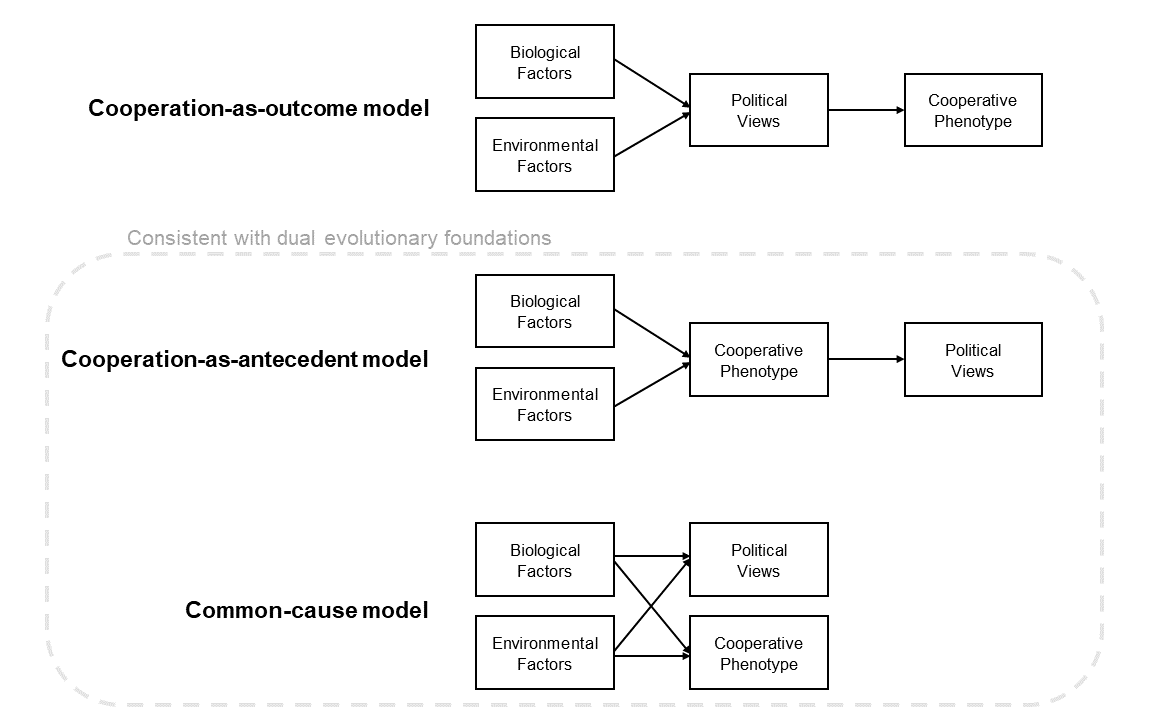
\includegraphics[width=\textwidth]{images/theoreticalModels} \caption{At least three theoretical causal models are
compatible with the cross-sectional correlation between political views and
the cooperative phenotype.}\label{fig:theoreticalModels}
\end{figure}

Longitudinal panel data allow us to generate specific hypotheses. If the
cooperation-as-outcome model is correct, then political views at time \emph{t} should
predict the cooperative phenotype at time \emph{t + 1}, but the cooperative phenotype
at time \emph{t} should be unrelated to political views at time \emph{t + 1}. If the
cooperation-as-antecedent model is correct, the opposite should be true: the
cooperative phenotype at time \emph{t} should predict political views at time
\emph{t + 1}, but political views at time \emph{t} should be unrelated to the cooperative
phenotype at time \emph{t + 1}. We further test whether a common cause is generating
the observed relationships by controlling for a wide range of plausible
demographic and personality confounds.

Here, we test between different causal hypotheses using a pre-registered
cross-lagged longitudinal panel design with two time-points separated by
eighteen months. We estimate the directions of causality between the cooperative
phenotype and several political views, including Social Dominance Orientation,
views on economic issues, and political party support.

\hypertarget{methods}{%
\section{Methods}\label{methods}}

\hypertarget{ethical-approval}{%
\subsection{Ethical approval}\label{ethical-approval}}

Ethical approval was granted by REDACTED (ref: 021666). The study was performed
in accordance with all the relevant guidelines and regulations. Participation
was voluntary and informed consent was obtained from all participants prior to
the study.

\hypertarget{participants-and-sampling}{%
\subsection{Participants and sampling}\label{participants-and-sampling}}

Participants were sampled from the New Zealand Attitudes and Values Study
(NZAVS), an annual longitudinal self-report study that has been active since
2009. 1045 participants took part in the first wave of economic game data
collection, were successfully paid for the study, and did not time out
of their session. In the second wave, this sample size dropped to 631
(60\% retention rate). Comparisons of drop-outs and non-drop-outs suggested that
retention did not systematically bias our sample (see Supplementary Table
\ref{tab:biasTable}). We only analysed data from participants who completed
both waves (n = 631;
411 females; mean age =
51 years; age range =
24 -
71 years). This sample size was
the largest available to us and was not determined through a formal power
analysis. These data are the same as used in our previous work
(Claessens, Kelly, Sibley, Chaudhuri, \& Atkinson, 2022; Claessens et al., 2023).

\hypertarget{materials}{%
\subsection{Materials}\label{materials}}

\hypertarget{self-report-measures}{%
\subsubsection{Self-report measures}\label{self-report-measures}}

Main self-report measures were taken from Waves 10 and 11 of the NZAVS. The
primary measures of interest for this study were: Social Dominance Orientation
(Pratto et al., 1994); support for income redistribution (``redistributing money and
wealth more evenly among a larger percentage of the people in New Zealand
through heavy taxes on the rich''); income attribution (``if incomes were more
equal, people would be less motivated to work hard''); and support for New
Zealand's centre-right National Party. We chose these measures because they all
exhibited cross-sectional correlations with the cooperative phenotype in
previous research (Claessens et al., 2023).

Other time-invariant covariates that could plausibly act as confounding
variables were taken from Wave 10 of the NZAVS. These included socio-demographic
variables (age, gender, ethnicity, education, local deprivation, socio-economic
status, and religiosity), personality variables (extraversion, agreeableness,
conscientiousness, neuroticism, openness-to-experience, honesty-humility, and
narcissism) (Sibley et al., 2011) and Right Wing Authoritarianism (Altemeyer, 1981). We
do not include RWA as a primary measure of interest in this study because our
previous work found no cross-sectional association between RWA and the
cooperative phenotype (Claessens et al., 2023). See Supplementary Table
\ref{tab:itemTable} for the full list of self-report items.

\hypertarget{battery-of-economic-games}{%
\subsubsection{Battery of economic games}\label{battery-of-economic-games}}

Participants completed three incentivised one-shot economic games, conducted
online in real-time using oTree software (Chen, Schonger, \& Wickens, 2016). These games measure
cooperative behaviour and are largely identical to the cooperation games used in
Peysakhovich et al. (2014). We used the strategy method to elicit responses in all roles.
Participants played for points, which were converted to New Zealand dollars
(1 point = \$0.035).

The three cooperation games are as follows:

\begin{itemize}
\tightlist
\item
  \emph{Dictator Game}. Player A is given 100 points. They must decide how many of
  these points to transfer to Player B. Player A keeps the remaining points.
  Player B is passive in the interaction.
\item
  \emph{Trust Game}. Players A and B both start with 50 points. First, Player A
  decides whether or not to transfer all 50 points to Player B, in the
  knowledge that the transferred amount will be tripled to 150 points. If
  Player A transfers, Player B now has 200 points. Player B must then decide to
  transfer 0 - 150 points back to Player A. There are thus two decisions in
  this game: giving and returning.
\item
  \emph{Public Goods Game}. Four players begin with 100 points each. They can
  contribute 0 - 100 points into a shared group project. All four decisions are
  made simultaneously, and then the amount in the group project is doubled and
  distributed evenly between all four players. Each player ends the game with
  their share from the group project, plus the points they initially refrained
  from contributing.
\end{itemize}

In both waves, participants also completed additional punishment games
(Ultimatum Game, Third Party Punishment Game, and Second Party Punishment Game).
Moreover, in the first wave, participants completed additional coordination
games (Stag Hunt Game and Stag Hunt Game with Punishment) and, in the second
wave, participants completed additional behavioural measures of rule following
and social information use (Claessens et al., 2023). We only used the Dictator Game,
Trust Game, and Public Goods Game to estimate the cooperative phenotype to be
consistent with prior research (Peysakhovich et al., 2014) and because these were the
only games for which prosocial behaviour (a) could be exploited by others and
(b) was not motivated by the threat of future punishment.

To determine whether learning occurred between waves and affected subsequent
game behaviour, we estimated differences in behaviour between the two waves (see
Supplementary Table \ref{tab:diffTable}). For the Public Goods Game and the
Trust Game, we found no differences in game behaviour between waves. In the
Dictator Game, participants gave slightly less in the second wave, but this
difference was small (2 fewer points given, on average, out of 100). These
results suggest that learning biases are not a major concern in our study.

\hypertarget{procedure}{%
\subsection{Procedure}\label{procedure}}

The NZAVS collects self-report data both online and via paper surveys. In Wave
10 of the study, most of the data were collected between November 2018 and
September 2019, and in Wave 11 of the study, most of the data were collected
between October 2019 and November 2020 (see Supplementary Figure
\ref{fig:timelinePlot} for timeline).

Data collection for the first wave of economic games was conducted between
18\textsuperscript{th} February and 25\textsuperscript{th} July 2019, and data collection for the second wave
was conducted between 19\textsuperscript{th} October and 11\textsuperscript{th} November 2020. Sessions were
conducted in real-time on midweek evenings, during which the economic games were
completed in a randomised order. Participants did not receive any information
about their earnings over the course of the session to avoid any potential
wealth or learning effects between games. See Supplementary Methods for further
procedural details.

After the sessions, participants were randomly matched into groups to determine
bonus payments. After being matched, participants were informed about their
outcomes in each of the economic games. Participants were paid a \$20 NZD
show-up fee, plus their bonus payment. In the first wave, participants earned a
bonus payment of \$25.27 on average (SD =
\$2.52). In the second wave, participants
earned a bonus payment of \$21.39 on
average (SD = \$2.63).

\hypertarget{pre-registration}{%
\subsection{Pre-registration}\label{pre-registration}}

We pre-registered our hypotheses on the Open Science Framework
(\url{https://osf.io/ksw3x/?view_only=597d9d552bc142f4a6d59e4eba97b425}) before
running the second wave of economic game data collection. First, we
hypothesised that the cooperation games in the second wave would all load onto
a single latent variable, replicating our previous work (Claessens et al., 2023).
Second, we hypothesised that this ``cooperative phenotype'' would be negatively
related to SDO within the second wave, again replicating our previous work.
Third, we hypothesised that the cooperative phenotype latent variable would
have at least scalar measurement invariance across waves (Carlsson, Johansson-Stenman, \& Nam, 2014; Peysakhovich et al., 2014). Fourth, we predicted that our longitudinal models would
provide support for at least one of the causal models visualised in Figure
\ref{fig:theoreticalModels}.

We deviated from our pre-registration in our interpretation of a lack of
cross-lagged effects. In the pre-registration, we stated that a lack of
cross-lagged effects, along with the presence of within-wave correlations, would
support the common-cause model in Figure \ref{fig:theoreticalModels}. However,
an anonymous reviewer pointed out that this is not necessarily true, especially
if potential common causes are not statistically controlled for. We no longer
make this statistical inference, but test several versions of the common cause
model by systematically controlling for a range of potential confounds,
including demographic and personality variables.

\hypertarget{statistical-analysis}{%
\subsection{Statistical analysis}\label{statistical-analysis}}

We used confirmatory factor analysis and structural equation modelling to test
our pre-registered hypotheses. For measurement invariance analyses, we fitted a
confirmatory factor analysis model with correlated item errors across waves to
deal with non-independence of observations. For our longitudinal modelling, we
used two-wave two-variable cross-lagged panel models.

86\% of participants had complete data
for all variables (see Supplementary Figure \ref{fig:plotObs}). To deal with
missing data, we used multiple imputation with predictive mean matching
(van Buuren \& Groothuis-Oudshoorn, 2011). Multiple imputation procedures generate a number of plausible
complete datasets with imputed missing values. Statistical models are then
fitted to all imputed datasets and results are pooled across models to account
for uncertainty in imputed values. We followed the advice of imputing at least
as many datasets as the percentage of cases that are incomplete
(Von Hippel, 2009). We therefore pooled our estimates across 20 imputed datasets.
Visual inspection confirmed the plausibility of imputed values (see
Supplementary Figure \ref{fig:impPlot}). Results for all models were
unchanged when using listwise deletion (see Supplementary Material).

\hypertarget{transparency-and-openness}{%
\subsection{Transparency and openness}\label{transparency-and-openness}}

Since the NZAVS is an ongoing longitudinal study, ethical concerns prevent us
from making the dataset from this study (including the main survey data and the
economic game data) publicly available. However, data are available on request
from the lead author.

Pre-registration, analysis plan, R code for analyses, and Python code for the
economic games are available at
\url{https://osf.io/ksw3x/?view_only=597d9d552bc142f4a6d59e4eba97b425}. All analyses
were conducted in R version 4.2.1 (R Core Team, 2019) using the \emph{lavaan} package
(Rosseel, 2012). Figures were created using \emph{ggraph} (Pedersen, 2020), \emph{cowplot}
(Wilke, 2019), and \emph{ggplot2} (Wickham, 2016) packages, multiple imputation was
implemented using the \emph{mice} package (van Buuren \& Groothuis-Oudshoorn, 2011), reproducibility of all analyses
was ensured by using the \emph{targets} package (Landau, 2021), and the manuscript was
generated using the \emph{papaja} package (Aust \& Barth, 2020).

\hypertarget{results}{%
\section{Results}\label{results}}

In the first step of our pre-registered analyses, we focused on the
second wave of data in order to replicate our previous findings from the first
wave (Claessens et al., 2023). First, we fitted a confirmatory factor analysis model
with the Trust Game (Give), Trust Game (Return), Dictator Game, and Public
Goods Game loading onto a ``cooperative phenotype'' latent variable. Supporting
our first pre-registered hypothesis, all factor loadings were significantly
positive (\emph{p} \textless{} 0.05) and the model fitted the data well (CFI =
0.99, RMSEA =
0.07, SRMR =
0.04; Supplementary Figure
\ref{fig:cfa1Plot}) (Hu \& Bentler, 1999; MacCallum, Browne, \& Sugawara, 1996). The games showed acceptable
reliability in both the first wave (\(\alpha\) =
0.61, \(\omega\) =
0.66) and the second wave (\(\alpha\) =
0.64, \(\omega\) =
0.70), and the zero-order correlations
between games were all positive and small-to-medium in size (\emph{r} = 0.20 -- 0.37;
Supplementary Figure \ref{fig:plotCors}) supporting the existence of a single
latent construct.

Second, we fitted a structural equation model with SDO as the sole predictor of
the cooperative phenotype latent variable. Supporting our second pre-registered
hypothesis, we found that SDO significantly negatively predicted the cooperative
phenotype (unstandardised \emph{b} = -0.13, 95\% confidence interval
{[}-0.20 -0.06{]}, \emph{p} \textless{} .001;
Supplementary Figure \ref{fig:sem1Plot}). Together, these findings replicate
our previous work with the same sample of participants eighteen months later
(Claessens et al., 2023).

In the next step of our pre-registered analyses, we tested the measurement
invariance of the cooperative phenotype latent variable across the two waves.
Longitudinal measurement invariance testing ensures that latent factor
structures are stable over time, an important prerequisite to cross-lagged
panel modelling. We found support for strict invariance of the cooperative
phenotype latent variable over time (see Supplementary Results) suggesting that
the cooperative phenotype was measured with the same reliability over an
eighteen-month period. Moreover, the between-wave latent correlation from the
strict invariance model (\emph{r} =
0.65, 95\% CI
{[}0.56
0.74{]}) suggested that the
cooperative phenotype exhibited good test-retest reliability over time.

We then proceeded to fit our pre-registered two-variable two-wave cross-lagged
panel models. We first fitted our primary cross-lagged panel model, modelling
the relationship between SDO and the cooperative phenotype over time (Figure
\ref{fig:clpmPlotASDO}a; Supplementary Figure \ref{fig:clpmPlotBSDO}a). We
found significantly positive autoregressive effects: SDO in the first wave
predicted SDO in the second wave (standardised
\(\beta\) = 0.81, unstandardised
\emph{b} = 0.84, 95\% CI {[}0.79
0.89{]}, \emph{p} \textless{} .001) and the cooperative phenotype
in the first wave predicted the cooperative phenotype in the second wave
(\(\beta\) = 0.65, \emph{b} =
0.73, 95\% CI {[}0.60 0.86{]},
\emph{p} \textless{} .001). Additionally, we found that the cooperative phenotype
in the first wave negatively predicted SDO in the second wave (\(\beta\) =
-0.09, \emph{b} =
-0.14, 95\% CI {[}-0.24 -0.04{]},
\emph{p} = .008), but SDO in the first wave did not predict the
cooperative phenotype in the second wave (\(\beta\)
= 0.00, \emph{b} =
0.00, 95\% CI {[}-0.03 0.03{]},
\emph{p} = .967). These cross-lagged paths were significantly
different from one another (difference in unstandardised estimates =
0.14, 95\% CI {[}0.03 0.24{]},
\emph{p} = .011). According to established benchmarks for cross-lagged
effect sizes, the cross-lagged effect of the cooperative phenotype on future SDO
is a medium-to-large effect size (Orth et al., 2022).

To test possible common-cause explanations for this pattern of results,
we ran additional cross-lagged panel models controlling for a range of
time-invariant covariates that could plausibly act as confounds (Figures
\ref{fig:clpmPlotASDO}b and \ref{fig:clpmPlotASDO}c; Supplementary Figures
\ref{fig:clpmPlotBSDO}b and \ref{fig:clpmPlotBSDO}c). The cross-lagged path
from the cooperative phenotype to later SDO remained significantly negative when
controlling for most demographic and personality variables, but was attenuated
when controlling for gender and ethnicity. Given these results, we ran
exploratory multi-group cross-lagged panel models with separate groups for (1)
male and female participants, and (2) participants of European ancestry and
participants not of European ancestry (due to small sample sizes in individual
Asian, Māori, and Pacific groups). These follow-up models revealed that the
cross-lagged path from the cooperative phenotype to later SDO was significantly
negative for males (\(\beta\) =
-0.12, \emph{b} =
-0.18, 95\% CI {[}-0.35
0.00{]}, \emph{p} = .044) but not for females
(\(\beta\) = -0.07, \emph{b} =
-0.10, 95\% CI {[}-0.22
0.02{]}, \emph{p} = .098) though these were both
in the same direction. Similarly, the cross-lagged path from the cooperative
phenotype to later SDO was significantly negative for participants of European
ancestry (\(\beta\) = -0.08,
\emph{b} = -0.13, 95\% CI {[}-0.25
-0.01{]}, \emph{p} = .028) but not for other
participants (\(\beta\) = -0.13,
\emph{b} = -0.17, 95\% CI {[}-0.37
0.02{]}, \emph{p} = .079) though these were both
in the same direction.











\begin{figure}
\centering
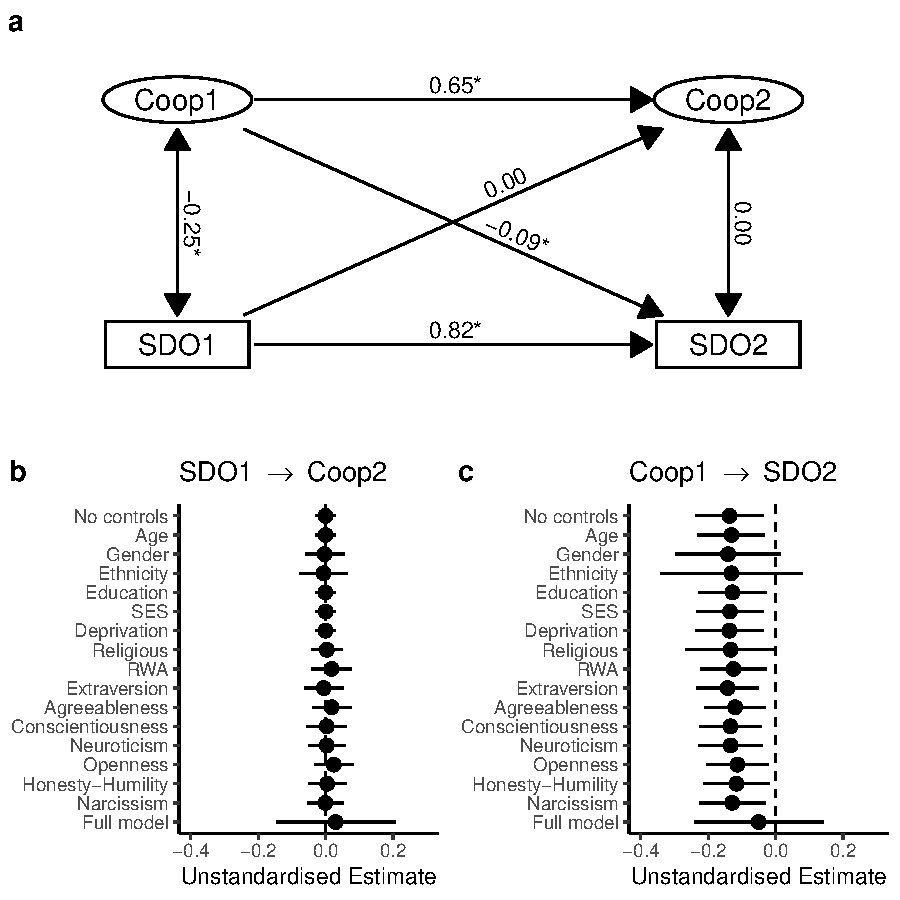
\includegraphics{manuscript_files/figure-latex/clpmPlotASDO-1.pdf}
\caption{\label{fig:clpmPlotASDO}\emph{Results of cross-lagged panel model with the
cooperative phenotype and SDO, pooling over 20 imputed datasets.} (a)
Autoregressive effects, cross-lagged effects, and within-wave (residual)
correlations from the model. Note that measurement models for the cooperative
phenotype latent variables are omitted from this figure. Numbers are
standardised coefficients, *\emph{p} \textless{} 0.05. (b, c) Forest plots visualising the
change in cross-lagged paths when controlling for time-invariant covariates,
individually and in a full model. Points are unstandardised estimates, lines
are 95\% confidence intervals.}
\end{figure}

We also collected data on other self-reported measures of political views,
including views on income redistribution, income attribution, and support for
the centre-right National Party. To assess the generalisability of our results,
we swapped out SDO in our cross-lagged panel model for these additional
measures.

When we included support for income redistribution in the model instead of SDO,
we found a similar pattern of results: the cooperative phenotype positively
predicted future support for income redistribution with a small-to-medium effect
size, but support for income redistribution did not predict future cooperation
(Supplementary Figures \ref{fig:clpmPlotAIncRed} and \ref{fig:clpmPlotBIncRed}).
However, this pattern of results was attenuated when controlling for gender,
ethnicity, religiosity, agreeableness, openness-to-experience, and
honesty-humility. When we included income attribution views and support for New
Zealand's centre-right National Party in the model instead of SDO, we found no
cross-lagged effects over time (Supplementary Figures \ref{fig:clpmPlotAIncAtt}
-- \ref{fig:clpmPlotBPolNat}).

\hypertarget{discussion}{%
\section{Discussion}\label{discussion}}

In a cross-lagged longitudinal analysis of cooperative behaviour and
self-reported political attitudes, we have shown that the cooperative phenotype
predicts SDO a year and a half later, but SDO does not predict future variation
in the cooperative phenotype. This result is in line with the
cooperation-as-antecedent model (Figure \ref{fig:theoreticalModels}) which
posits that general behavioural predispositions like the cooperative phenotype
causally influence political views, but not vice versa. This causal model
explains previously reported negative cross-sectional correlations between
cooperation and SDO (Claessens et al., 2023; Haesevoets et al., 2018, 2015; Halali et al., 2018; Thielmann et al., 2020) as arising from a causal relationship from
behavioural preferences to political views.

Additionally, the cross-lagged path from cooperation to future SDO was robust
to a wide range of time-invariant demographic and personality covariates. It is
therefore unlikely that these variables are acting as common causes and
generating the observed pattern of relationships (though, of course, it remains
possible that other unmodelled common causes could exist). However, the
cross-lagged path from cooperation to future SDO was attenuated when controlling
for gender and ethnicity. In particular, exploratory analyses revealed that the
cross-lagged effect held only for male participants of European ancestry. This
is similar to the finding that upper body strength is related to support for
inequality in males, but not females (Petersen \& Laustsen, 2019). A possible evolutionary
explanation for this effect of gender might be that humans have large sexual
dimorphism in strength and formidability and, therefore, a correlation between
the cooperative phenotype and dominative/competitive tactics for resource
distribution is more likely among males. But this does not explain the effect of
ethnicity. Perhaps a simpler explanation is that SDO is generally higher among
males and people from dominant ethnic groups (Pratto et al., 1994; Sidanius, Levin, Liu, \& Pratto, 2000). Among
these participants, there is potentially more room for a change in SDO over
time, whereas female participants from minority ethnic groups may have already
hit the floor of the scale and therefore have less room for change. In line with
this explanation, when we look at the differences in SDO between the two waves,
we find that these difference scores have a higher variance for males of
European ancestry (variance = 0.39) compared to other
participants (variance = 0.24; Levene's test,
\emph{F}(1,564) = 13.54,
\emph{p} \textless{} .001) suggesting that SDO had more room for
change over time among males of European ancestry. Future research should
disentangle the roles of gender and ethnicity in the causal relationship
between behavioural predispositions and political views.

When we generalised our cross-lagged analysis to other political views, we found
more mixed results. As expected, the cooperative phenotype positively predicted
future support for income redistribution, but cooperation was not longitudinally
related to support for the centre-right National Party, nor was it
longitudinally related to income attribution beliefs. These null results could
arise from a shared cause influencing these variables at the same time (i.e.,
the common-cause model in Figure \ref{fig:theoreticalModels}) creating a
cross-sectional relationship but no longitudinal effects. However, this pattern
of null results is also consistent with other explanations. For example, it may
be that party affiliation and income attribution beliefs are simply less
amenable to change over time: people rarely shift their political party
affiliation (Pew Research Center, 2020) and income attribution beliefs have been
characterised as a stable individual difference (Osborne \& Weiner, 2015; but see Piff et al., 2020). Alternatively, cross-lagged effects may exist between the
cooperative phenotype and these variables but on longer or shorter timescales
than studied here. It is therefore difficult to interpret these null results
as supporting any particular causal model from Figure
\ref{fig:theoreticalModels}.

Nevertheless, our results for SDO and views on income redistribution are broadly
consistent with the dual evolutionary foundations framework for political
ideology. The cross-lagged effects of the cooperative phenotype on these
variables support either the cooperation-as-antecedent or common cause model,
and none of our results directly support the causal model that is inconsistent
with the dual evolutionary foundations (the cooperation-as-outcome model).
Moreover, our measurement invariance analyses and the latent correlation from
our strict invariance model revealed that the cooperative phenotype latent
variable had adequate test-retest reliability over eighteen months, supporting
another central claim from the dual evolutionary foundations framework that the
general social drives that partly shape political ideology should be relatively
stable over time. This finding expands on studies showing that cooperative
behaviour in individual economic games positively covaries when measured over
four months (Peysakhovich et al., 2014; Reigstad et al., 2017), one year (Lönnqvist, Verkasalo, Walkowitz, \& Wichardt, 2015), and
even six years (Carlsson et al., 2014).

One important limitation of this study is our use of two-wave cross-lagged
panel models to determine longitudinal effects. Cross-lagged panel models have
been criticised for not correctly partitioning within-person change from stable
between-person differences (Hamaker, Kuiper, \& Grasman, 2015). As an alternative to the
cross-lagged panel model, Hamaker et al. (2015) proposed the random-intercept
cross-lagged panel model, which estimates a random intercept to capture stable
individual differences over time. Unfortunately, random-intercept cross-lagged
panel models require at least three waves of data to be identified
(Hamaker et al., 2015) and so we were limited by our two waves of data in this study.
Moving forward, it will be vital to extend this study to include additional
waves of behavioural and self-report data to determine if our results hold when
accounting for stable between-person differences.

Future research should expand our multi-wave behavioural and self-report
approach to include additional measures. In particular, to provide a complete
picture for the dual evolutionary foundations framework, future research should
test whether group conformist predispositions predict future variation in RWA
and social policy views. Evidence already suggests that RWA covaries
cross-sectionally with conformist behaviour in the rule following task and
social learning tasks (Claessens et al., 2023; Fischer, Atkinson, \& Chaudhuri, 2021). Extending this research
longitudinally will allow researchers to make stronger causal inferences than
are possible on the basis of cross-sectional data alone. We hope that future
work will continue to unpack the causal pathways underlying the psychological
causes and consequences of political ideology.

\newpage
\nolinenumbers

\hypertarget{acknowledgements}{%
\section{Acknowledgements}\label{acknowledgements}}

This work was supported by a Royal Society of New Zealand Marsden Grant
(REDACTED). The New Zealand Attitudes and Values Study is funded by a grant
from the Templeton Religion Trust (REDACTED).

\hypertarget{author-contributions}{%
\section{Author Contributions}\label{author-contributions}}

All authors conceived of and designed the study. REDACTED collected behavioural
data and conducted all statistical analyses. REDACTED managed survey data
collection. REDACTED wrote the paper with input from REDACTED.

\hypertarget{competing-interests}{%
\section{Competing Interests}\label{competing-interests}}

The authors declare no competing interests.

\newpage

\hypertarget{references}{%
\section{References}\label{references}}

\begingroup

\hypertarget{refs}{}
\begin{CSLReferences}{1}{0}
\leavevmode\vadjust pre{\hypertarget{ref-Altemeyer1981}{}}%
Altemeyer, B. (1981). \emph{Right-wing authoritarianism}. University of Manitoba Press.

\leavevmode\vadjust pre{\hypertarget{ref-R-papaja}{}}%
Aust, F., \& Barth, M. (2020). \emph{{papaja}: {Create} {APA} manuscripts with {R Markdown}}. Retrieved from \url{https://github.com/crsh/papaja}

\leavevmode\vadjust pre{\hypertarget{ref-Brandt2014}{}}%
Brandt, M. J., Reyna, C., Chambers, J. R., Crawford, J. T., \& Wetherell, G. (2014). The ideological-conflict hypothesis: Intolerance among both liberals and conservatives. \emph{Current Directions in Psychological Science}, \emph{23}(1), 27--34. \url{https://doi.org/10.1177/0963721413510932}

\leavevmode\vadjust pre{\hypertarget{ref-Campbell1960}{}}%
Campbell, A., Converse, P. E., Miller, W. E., \& Stokes, D. E. (1960). \emph{The {A}merican voter}. Chicago: Wiley.

\leavevmode\vadjust pre{\hypertarget{ref-Carlsson2014}{}}%
Carlsson, F., Johansson-Stenman, O., \& Nam, P. K. (2014). Social preferences are stable over long periods of time. \emph{Journal of Public Economics}, \emph{117}, 104--114. https://doi.org/\url{https://doi.org/10.1016/j.jpubeco.2014.05.009}

\leavevmode\vadjust pre{\hypertarget{ref-Chen2016}{}}%
Chen, D. L., Schonger, M., \& Wickens, C. (2016). {oTree}-an open-source platform for laboratory, online, and field experiments. \emph{Journal of Behavioral and Experimental Finance}, \emph{9}, 88--97. \url{https://doi.org/10.1016/j.jbef.2015.12.001}

\leavevmode\vadjust pre{\hypertarget{ref-Chierchia2017}{}}%
Chierchia, G., Lesemann, F. P., Snower, D., Vogel, M., \& Singer, T. (2017). Caring cooperators and powerful punishers: Differential effects of induced care and power motivation on different types of economic decision making. \emph{Scientific Reports}, \emph{7}(1), 11068.

\leavevmode\vadjust pre{\hypertarget{ref-Chirumbolo2016}{}}%
Chirumbolo, A., Leone, L., \& Desimoni, M. (2016). The interpersonal roots of politics: Social value orientation, socio-political attitudes and prejudice. \emph{Personality and Individual Differences}, \emph{91}, 144--153.

\leavevmode\vadjust pre{\hypertarget{ref-Claessens2020}{}}%
Claessens, S., Fischer, K., Chaudhuri, A., Sibley, C. G., \& Atkinson, Q. D. (2020). The dual evolutionary foundations of political ideology. \emph{Nature Human Behaviour}, \emph{4}, 336--345. \url{https://doi.org/10.1038/s41562-020-0850-9}

\leavevmode\vadjust pre{\hypertarget{ref-Claessens2022}{}}%
Claessens, S., Kelly, D., Sibley, C. G., Chaudhuri, A., \& Atkinson, Q. D. (2022). Cooperative phenotype predicts climate change belief and pro-environmental behaviour. \emph{Scientific Reports}, \emph{12}(1), 12730.

\leavevmode\vadjust pre{\hypertarget{ref-Claessens2023}{}}%
Claessens, S., Sibley, C. G., Chaudhuri, A., \& Atkinson, Q. D. (2023). Cooperative and conformist behavioural preferences predict the dual dimensions of political ideology. \emph{Scientific Reports}, \emph{13}(1), 4886.

\leavevmode\vadjust pre{\hypertarget{ref-Duckitt2009}{}}%
Duckitt, J., \& Sibley, C. G. (2009). A dual-process motivational model of ideology, politics, and prejudice. \emph{Psychological Inquiry}, \emph{20}(2-3), 98--109. \url{https://doi.org/10.1080/10478400903028540}

\leavevmode\vadjust pre{\hypertarget{ref-Fischer2021}{}}%
Fischer, K., Atkinson, Q. D., \& Chaudhuri, A. (2021). Experiments in political psychology. In A. Chaudhuri (Ed.), \emph{A research agenda for experimental economics}. Cheltenham: Edward Elgar.

\leavevmode\vadjust pre{\hypertarget{ref-Grunhage2020}{}}%
Grünhage, T., \& Reuter, M. (2020). Political orientation is associated with behavior in public-goods- and trust-games. \emph{Political Behavior}, (0123456789). \url{https://doi.org/10.1007/s11109-020-09606-5}

\leavevmode\vadjust pre{\hypertarget{ref-Haesevoets2018}{}}%
Haesevoets, T., Reinders Folmer, C., Bostyn, D. H., \& Van Hiel, A. (2018). Behavioural consistency within the prisoner's dilemma game: The role of personality and situation. \emph{European Journal of Personality}, \emph{32}(4), 405--426. \url{https://doi.org/10.1002/per.2158}

\leavevmode\vadjust pre{\hypertarget{ref-Haesevoets2015}{}}%
Haesevoets, T., Reinders Folmer, C., \& Van Hiel, A. (2015). Cooperation in mixed-motive games: The role of individual differences in selfish and social orientation. \emph{European Journal of Personality}, \emph{29}(4), 445--458. \url{https://doi.org/10.1002/per.1992}

\leavevmode\vadjust pre{\hypertarget{ref-Halali2018}{}}%
Halali, E., Dorfman, A., Jun, S., \& Halevy, N. (2018). More for us or more for me? Social dominance as parochial egoism. \emph{Social Psychological and Personality Science}, \emph{9}(2), 254--262. \url{https://doi.org/10.1177/1948550617732819}

\leavevmode\vadjust pre{\hypertarget{ref-Hamaker2015}{}}%
Hamaker, E. L., Kuiper, R. M., \& Grasman, R. P. P. P. (2015). A critique of the cross-lagged panel model. \emph{Psychological Methods}, \emph{20}(1), 102.

\leavevmode\vadjust pre{\hypertarget{ref-Hu1999}{}}%
Hu, L. T., \& Bentler, P. M. (1999). Cutoff criteria for fit indexes in covariance structure analysis: Conventional criteria versus new alternatives. \emph{Structural Equation Modeling}, \emph{6}(1), 1--55. \url{https://doi.org/10.1080/10705519909540118}

\leavevmode\vadjust pre{\hypertarget{ref-Inbar2012}{}}%
Inbar, Y., Pizarro, D., Iyer, R., \& Haidt, J. (2012). Disgust sensitivity, political conservatism, and voting. \emph{Social Psychological and Personality Science}, \emph{3}(5), 537--544.

\leavevmode\vadjust pre{\hypertarget{ref-Jost2009}{}}%
Jost, J. T., Federico, C. M., \& Napier, J. L. (2009). Political ideology: Its structure, functions, and elective affinities. \emph{Annual Review of Psychology}, \emph{60}(1), 307--337. \url{https://doi.org/10.1146/annurev.psych.60.110707.163600}

\leavevmode\vadjust pre{\hypertarget{ref-Jost2003}{}}%
Jost, J. T., Glaser, J., Kruglanski, A. W., \& Sulloway, F. J. (2003). Political conservatism as motivated social cognition. \emph{Psychological Bulletin}, \emph{129}(3), 339--375.

\leavevmode\vadjust pre{\hypertarget{ref-R-targets}{}}%
Landau, W. M. (2021). The targets {R} package: A dynamic {M}ake-like function-oriented pipeline toolkit for reproducibility and high-performance computing. \emph{Journal of Open Source Software}, \emph{6}(57), 2959. Retrieved from \url{https://doi.org/10.21105/joss.02959}

\leavevmode\vadjust pre{\hypertarget{ref-Lonnqvist2015}{}}%
Lönnqvist, J.-E., Verkasalo, M., Walkowitz, G., \& Wichardt, P. C. (2015). Measuring individual risk attitudes in the lab: Task or ask? An empirical comparison. \emph{Journal of Economic Behavior \& Organization}, \emph{119}, 254--266. https://doi.org/\url{https://doi.org/10.1016/j.jebo.2015.08.003}

\leavevmode\vadjust pre{\hypertarget{ref-MacCallum1996}{}}%
MacCallum, R. C., Browne, M. W., \& Sugawara, H. M. (1996). Power analysis and determination of sample size for covariance structure modeling. \emph{Psychological Methods}, \emph{1}(2), 130--149. \url{https://doi.org/10.1037/1082-989x.1.2.130}

\leavevmode\vadjust pre{\hypertarget{ref-Orth2022}{}}%
Orth, U., Meier, L. L., Bühler, J. L., Dapp, L. C., Krauss, S., Messerli, D., \& Robins, R. W. (2022). Effect size guidelines for cross-lagged effects. \emph{Psychological Methods}. \url{https://doi.org/10.1037/met0000499}

\leavevmode\vadjust pre{\hypertarget{ref-Osborne2020}{}}%
Osborne, D., \& Sibley, C. G. (2020). Does openness to experience predict changes in conservatism? A nine-wave longitudinal investigation into the personality roots to ideology. \emph{Journal of Research in Personality}, \emph{87}, 103979. \url{https://doi.org/10.1016/j.jrp.2020.103979}

\leavevmode\vadjust pre{\hypertarget{ref-Osborne2015}{}}%
Osborne, D., \& Weiner, B. (2015). A latent profile analysis of attributions for poverty: Identifying response patterns underlying people's willingness to help the poor. \emph{Personality and Individual Differences}, \emph{85}, 149--154. https://doi.org/\url{https://doi.org/10.1016/j.paid.2015.05.007}

\leavevmode\vadjust pre{\hypertarget{ref-R-ggraph}{}}%
Pedersen, T. L. (2020). \emph{{ggraph}: An implementation of grammar of graphics for graphs and networks}. Retrieved from \url{https://CRAN.R-project.org/package=ggraph}

\leavevmode\vadjust pre{\hypertarget{ref-Petersen2019}{}}%
Petersen, M. B., \& Laustsen, L. (2019). Upper-body strength and political egalitarianism: Twelve conceptual replications. \emph{Political Psychology}, \emph{40}(2), 375--394. https://doi.org/\url{https://doi.org/10.1111/pops.12505}

\leavevmode\vadjust pre{\hypertarget{ref-PewResearchCenter2020}{}}%
Pew Research Center. (2020). \emph{Voters rarely switch parties, but recent shifts further educational, racial divergence}. Retrieved from \url{https://www.pewresearch.org/politics/2020/08/04/voters-rarely-switch-parties-but-recent-shifts-further-educational-racial-divergence/}

\leavevmode\vadjust pre{\hypertarget{ref-Peysakhovich2014}{}}%
Peysakhovich, A., Nowak, M. A., \& Rand, D. G. (2014). Humans display a {``cooperative phenotype''} that is domain general and temporally stable. \emph{Nature Communications}, \emph{5}, 4939. \url{https://doi.org/10.1038/ncomms5939}

\leavevmode\vadjust pre{\hypertarget{ref-Piff2020}{}}%
Piff, P. K., Wiwad, D., Robinson, A. R., Aknin, L. B., Mercier, B., \& Shariff, A. (2020). Shifting attributions for poverty motivates opposition to inequality and enhances egalitarianism. \emph{Nature Human Behaviour}, \emph{4}(5), 496--505. \url{https://doi.org/10.1038/s41562-020-0835-8}

\leavevmode\vadjust pre{\hypertarget{ref-Pisor2020}{}}%
Pisor, A. C., Gervais, M. M., Purzycki, B. G., \& Ross, C. T. (2020). Preferences and constraints: The value of economic games for studying human behaviour. \emph{Royal Society Open Science}, \emph{7}(6), 192090. \url{https://doi.org/10.1098/rsos.192090}

\leavevmode\vadjust pre{\hypertarget{ref-Pratto1994}{}}%
Pratto, F., Sidanius, J., Stallworth, L. M., \& Malle, B. F. (1994). Social dominance orientation: A personality variable predicting social and political attitudes. \emph{Journal of Personality and Social Psychology}, \emph{67}(4), 741.

\leavevmode\vadjust pre{\hypertarget{ref-R-base}{}}%
R Core Team. (2019). \emph{{R: A Language and Environment for Statistical Computing}}. Vienna, Austria: R Foundation for Statistical Computing. Retrieved from \url{https://www.R-project.org/}

\leavevmode\vadjust pre{\hypertarget{ref-Reigstad2017}{}}%
Reigstad, A. G., Strømland, E. A., \& Tinghög, G. (2017). Extending the cooperative phenotype: Assessing the stability of cooperation across countries. \emph{Frontiers in Psychology}, \emph{8}, 1990. \url{https://doi.org/10.3389/fpsyg.2017.01990}

\leavevmode\vadjust pre{\hypertarget{ref-R-lavaan}{}}%
Rosseel, Y. (2012). {lavaan}: An {R} package for structural equation modeling. \emph{Journal of Statistical Software}, \emph{48}(2), 1--36. Retrieved from \url{http://www.jstatsoft.org/v48/i02/}

\leavevmode\vadjust pre{\hypertarget{ref-Sibley2011}{}}%
Sibley, C. G., Luyten, N., Purnomo, M., Mobberley, A., Wootton, L. W., Hammond, M. D., et al.others. (2011). The {M}ini-{IPIP}6: Validation and extension of a short measure of the {B}ig-{S}ix factors of personality in {N}ew {Z}ealand. \emph{New Zealand Journal of Psychology (Online)}, \emph{40}(3), 142.

\leavevmode\vadjust pre{\hypertarget{ref-Sidanius2000}{}}%
Sidanius, J., Levin, S., Liu, J., \& Pratto, F. (2000). Social dominance orientation, anti-egalitarianism and the political psychology of gender: An extension and cross-cultural replication. \emph{European Journal of Social Psychology}, \emph{30}(1), 41--67.

\leavevmode\vadjust pre{\hypertarget{ref-Thielmann2022}{}}%
Thielmann, I., Hilbig, B. E., \& Zettler, I. (2022). The dispositional basis of human prosociality. \emph{Current Opinion in Psychology}, \emph{43}, 289--294.

\leavevmode\vadjust pre{\hypertarget{ref-Thielmann2020}{}}%
Thielmann, I., Spadaro, G., \& Balliet, D. (2020). Personality and prosocial behavior: A theoretical framework and meta-analysis. \emph{Psychological Bulletin}, \emph{146}(1), 30--90. \url{https://doi.org/10.1037/bul0000217}

\leavevmode\vadjust pre{\hypertarget{ref-Tomasello2012}{}}%
Tomasello, M., Melis, A. P., Tennie, C., Wyman, E., \& Herrmann, E. (2012). Two key steps in the evolution of human cooperation: The interdependence hypothesis. \emph{Current Anthropology}, \emph{53}(6), 673--692. \url{https://doi.org/10.1086/668207}

\leavevmode\vadjust pre{\hypertarget{ref-R-mice}{}}%
van Buuren, S., \& Groothuis-Oudshoorn, K. (2011). {mice}: Multivariate imputation by chained equations in {R}. \emph{Journal of Statistical Software}, \emph{45}(3), 1--67. Retrieved from \url{https://www.jstatsoft.org/v45/i03/}

\leavevmode\vadjust pre{\hypertarget{ref-VanLange2012}{}}%
Van Lange, P. A. M., Bekkers, R., Chirumbolo, A., \& Leone, L. (2012). Are conservatives less likely to be prosocial than liberals? From games to ideology, political preferences and voting. \emph{European Journal of Personality}, \emph{26}(5), 461--473. \url{https://doi.org/10.1002/per.845}

\leavevmode\vadjust pre{\hypertarget{ref-vonHippel2009}{}}%
Von Hippel, P. T. (2009). How to impute interactions, squares, and other transformed variables. \emph{Sociological Methodology}, \emph{39}(1), 265--291. \url{https://doi.org/10.1111/j.1467-9531.2009.01215.x}

\leavevmode\vadjust pre{\hypertarget{ref-R-ggplot2}{}}%
Wickham, H. (2016). \emph{{ggplot2: Elegant Graphics for Data Analysis}}. Springer-Verlag New York. Retrieved from \url{https://ggplot2.tidyverse.org}

\leavevmode\vadjust pre{\hypertarget{ref-R-cowplot}{}}%
Wilke, C. O. (2019). \emph{{cowplot: Streamlined Plot Theme and Plot Annotations for {``ggplot2''}}}. Retrieved from \url{https://CRAN.R-project.org/package=cowplot}

\leavevmode\vadjust pre{\hypertarget{ref-Yamagishi2013}{}}%
Yamagishi, T., Mifune, N., Li, Y., Shinada, M., Hashimoto, H., Horita, Y., et al.others. (2013). Is behavioral pro-sociality game-specific? Pro-social preference and expectations of pro-sociality. \emph{Organizational Behavior and Human Decision Processes}, \emph{120}(2), 260--271.

\leavevmode\vadjust pre{\hypertarget{ref-Zaller1992}{}}%
Zaller, J. R. (1992). \emph{The nature and origins of mass opinion}. Cambridge, UK: Cambridge University Press. \url{https://doi.org/10.1017/CBO9780511818691}

\end{CSLReferences}

\endgroup
\newpage
\vspace*{60mm}

\renewcommand{\figurename}{Supplementary Figure}
\renewcommand{\tablename}{Supplementary Table}
\renewcommand{\thefigure}{\arabic{figure}} \setcounter{figure}{0}
\renewcommand{\thetable}{\arabic{table}} \setcounter{table}{0}
\renewcommand{\theequation}{\arabic{equation}} \setcounter{equation}{0}

\hypertarget{supplementary-information}{%
\section{\texorpdfstring{\textbf{Supplementary Information}}{Supplementary Information}}\label{supplementary-information}}

\setcounter{page}{1}
\centering

\noindent \footnotesize Cooperative phenotype predicts political views on hierarchy and redistribution eighteen months later \newline
\hspace*{8mm} \footnotesize Scott Claessens\textsuperscript{1}, Chris G Sibley\textsuperscript{1}, Ananish Chaudhuri\textsuperscript{2,3}, \& Quentin D Atkinson\textsuperscript{1,4} \newline

\raggedright

\noindent \footnotesize \textsuperscript{1} School of Psychology, University of Auckland, New Zealand \newline
\noindent \footnotesize \textsuperscript{2} Department of Economics, University of Auckland, Auckland, New Zealand \newline
\noindent \footnotesize \textsuperscript{3} CESifo, Munich, Germany \newline
\noindent \footnotesize \textsuperscript{4} Max Planck Institute for the Science of Human History, Jena, Germany \newline
\normalsize
\newpage

\hypertarget{supplementary-methods}{%
\subsection{Supplementary Methods}\label{supplementary-methods}}

\hypertarget{procedure-for-economic-game-sessions}{%
\subsubsection{Procedure for economic game sessions}\label{procedure-for-economic-game-sessions}}

In both waves, participants were booked into sessions on midweek evenings and
completed the session online in real-time. Session sizes varied between 14 and
130 participants. Although participants knew they were completing the study with
other participants from the New Zealand Attitudes and Values Study, they did not
know specifically who they were interacting with in the session or how many
other people there were in the session.

Participants completed a consent form before proceeding to the eight
behavioural tasks (three cooperation games described in the main text, plus
additional tasks). In the first wave, all eight tasks were completed in a
randomised order. In the second wave, the economic games shared with the first
wave were completed first in a randomised order, followed by two new tasks (the
rule following and social information use tasks) which were presented in a
separately randomised order. For each task, participants read the instructions
for the task, completed a comprehension question, and then proceeded to make
their decisions.

After making their decisions for all the tasks, participants entered a waiting
lobby in which they waited for all other participants in their session to
complete the tasks. If participants took longer than 55 minutes to complete the
tasks, they were skipped ahead to the waiting lobby. Timeouts were still paid
their show-up fee, but not their bonus. In the first wave, participants took
22 minutes on average to
complete all eight tasks (SD =
7 minutes, range =
9 -
47
minutes), and in the second wave, participants took
24
minutes on average (SD = 8
minutes, range = 9 -
49 minutes).

\newpage

\hypertarget{supplementary-results}{%
\subsection{Supplementary Results}\label{supplementary-results}}

\hypertarget{measurement-invariance-results}{%
\subsubsection{Measurement invariance results}\label{measurement-invariance-results}}

We tested for measurement invariance of the cooperative phenotype factor
structure in a series of increasingly restrictive nested models. For all model
comparisons, we pre-registered the use of changes in fit statistics as
thresholds for diagnosing reduced model fit
{[}\(\Delta\)Comparative Fit Index (CFI) \textless{} -0.01, \(\Delta\)Root Mean Square Error of
Approximation (RMSEA) \textgreater{} 0.015{]} rather than \(\chi^2\) differences which are
sensitive to large sample sizes. To deal with non-independence of observations,
all measurement invariance models had correlated item errors across waves.

First, we fitted a configural invariance model, which freely estimated the two
latent variables simultaneously (Supplementary Table \ref{tab:tableCompareMI}).
As expected, this configural invariance model fitted the data well (CFI =
0.99, RMSEA =
0.04) and all loadings were
significantly positive. Second, we fitted a metric invariance model, which
constrained the item loadings to equality across the two waves. Model fit did
not substantially change (\(\Delta\)CFI =
-0.006,
\(\Delta\)RMSEA =
0.006).
Third, we fitted a scalar invariance model, which constrained the item
loadings, intercepts, and thresholds to equality across the two waves. Again,
model fit did not substantially change (\(\Delta\)CFI =
0.000,
\(\Delta\)RMSEA =
-0.004).
Fourth, and finally, we fitted a strict invariance model, which constrained the
item loadings, intercepts, thresholds, and variances to equality across waves.
Model fit remained unchanged (\(\Delta\)CFI =
0.000,
\(\Delta\)RMSEA =
-0.002).
Measurement invariance analysis thus supports strict invariance of the
cooperative phenotype latent variable over time.

\newpage

\hypertarget{supplementary-figures}{%
\subsection{Supplementary Figures}\label{supplementary-figures}}






\begin{figure}
\centering
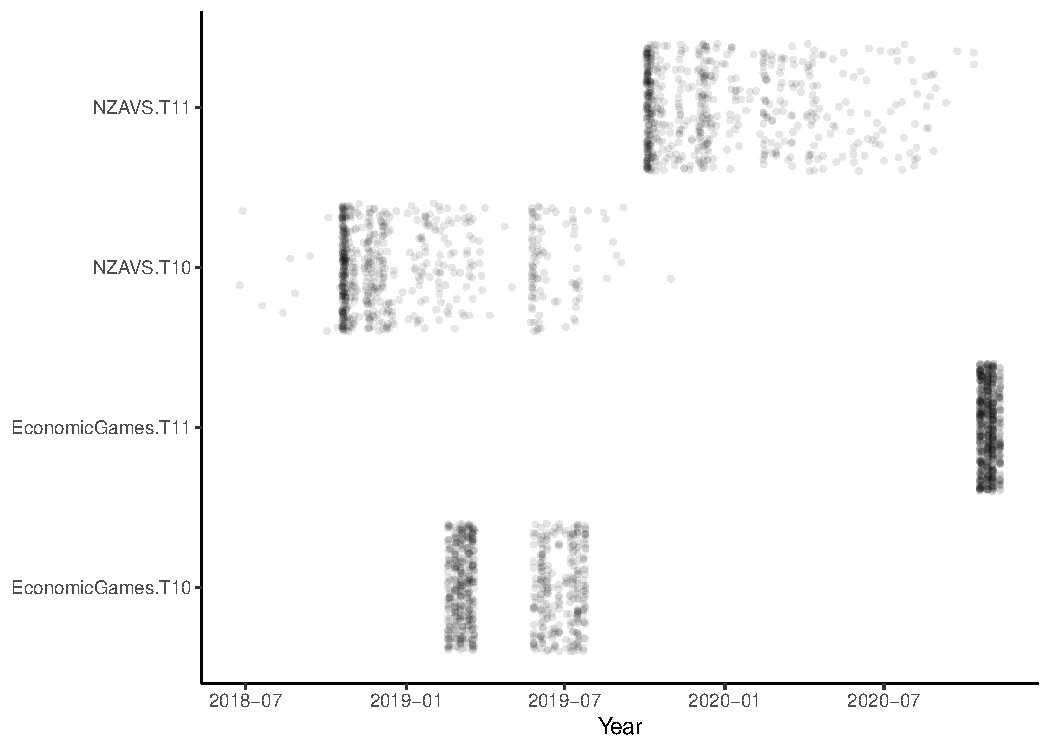
\includegraphics{manuscript_files/figure-latex/timelinePlot-1.pdf}
\caption{\label{fig:timelinePlot}\emph{Data collection timeline for NZAVS Wave 10, NZAVS
Wave 11, and both waves of economic game data collection (n = 631).} Each point is an individual participant. Note
the break in data collection in February 2019 due to the Christchurch
terrorist attack.}
\end{figure}

\newpage




\begin{figure}
\centering
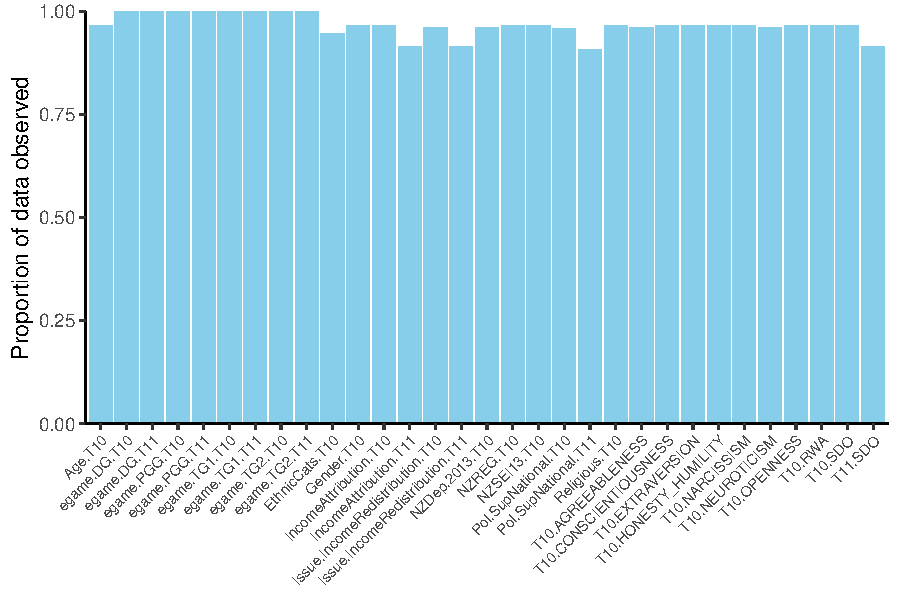
\includegraphics{manuscript_files/figure-latex/plotObs-1.pdf}
\caption{\label{fig:plotObs}\emph{Bar plot showing proportions of observed data for all
variables included in the study}. T10 = NZAVS Wave 10, T11 = NZAVS Wave 11.}
\end{figure}

\newpage





\begin{figure}
\centering
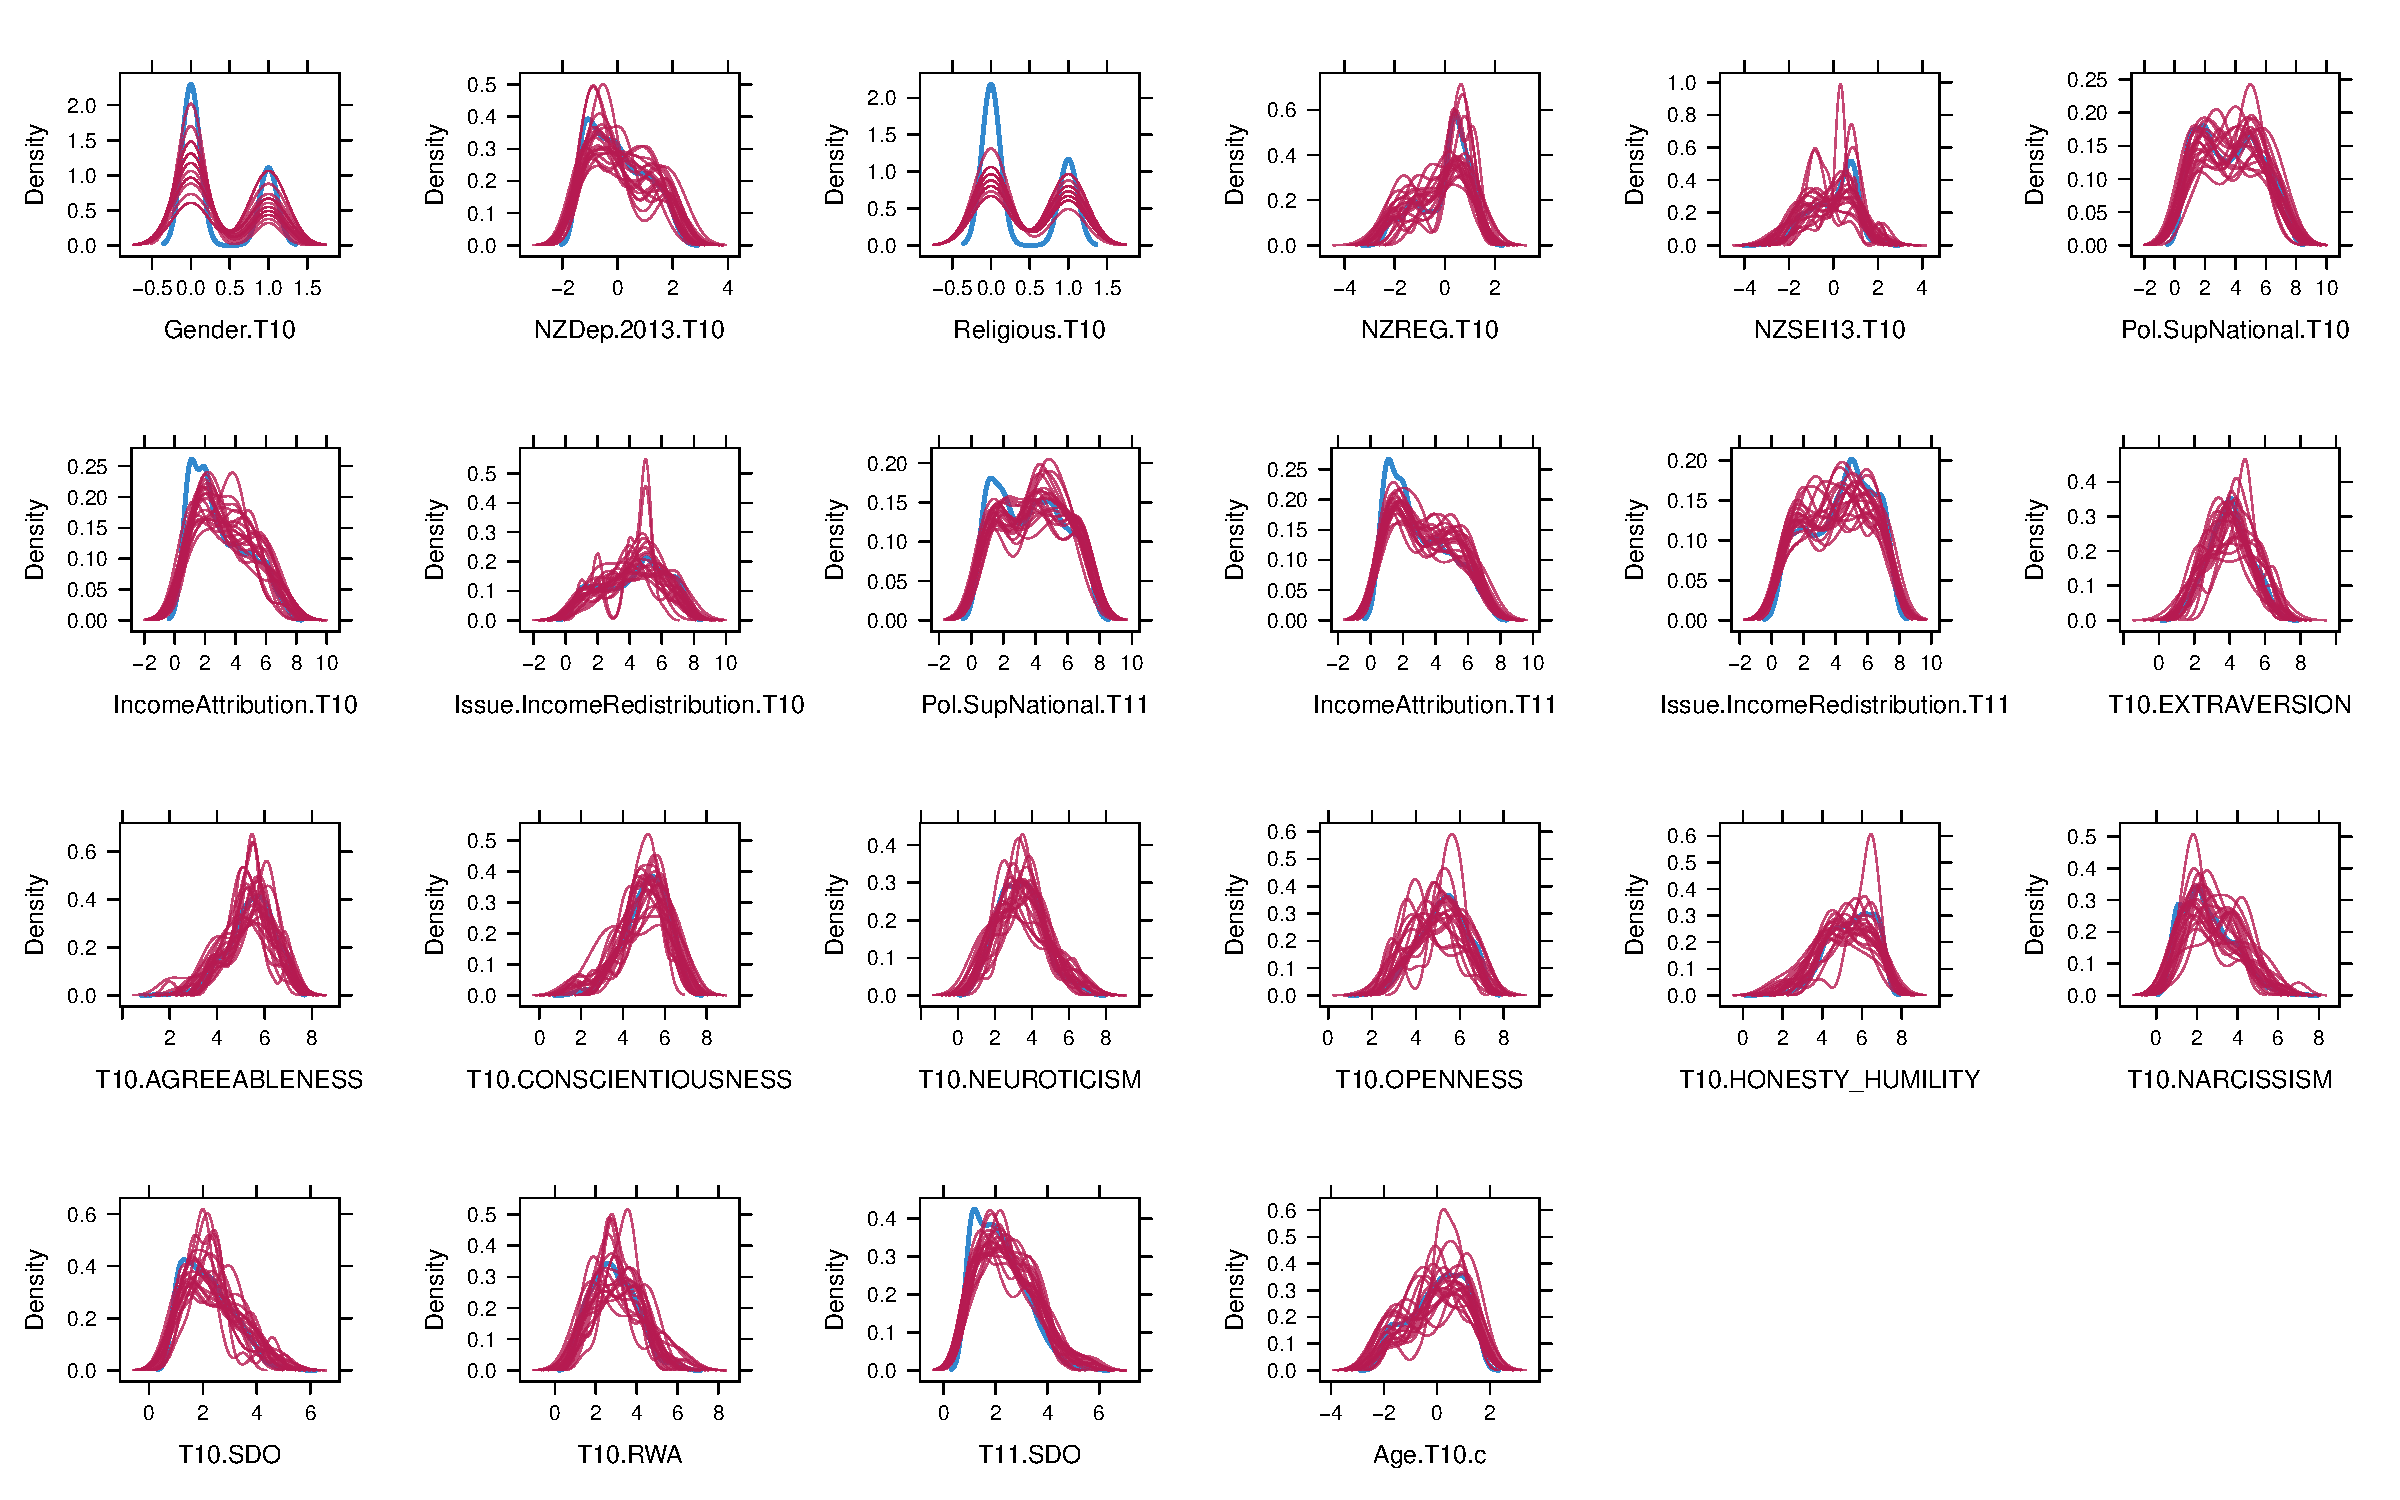
\includegraphics{manuscript_files/figure-latex/impPlot-1.pdf}
\caption{\label{fig:impPlot}\emph{Density plots showing imputed values from 20 multiply
imputed datasets (pink) against observed values (blue).} Data were imputed
using predictive mean matching.}
\end{figure}

\newpage






\begin{figure}
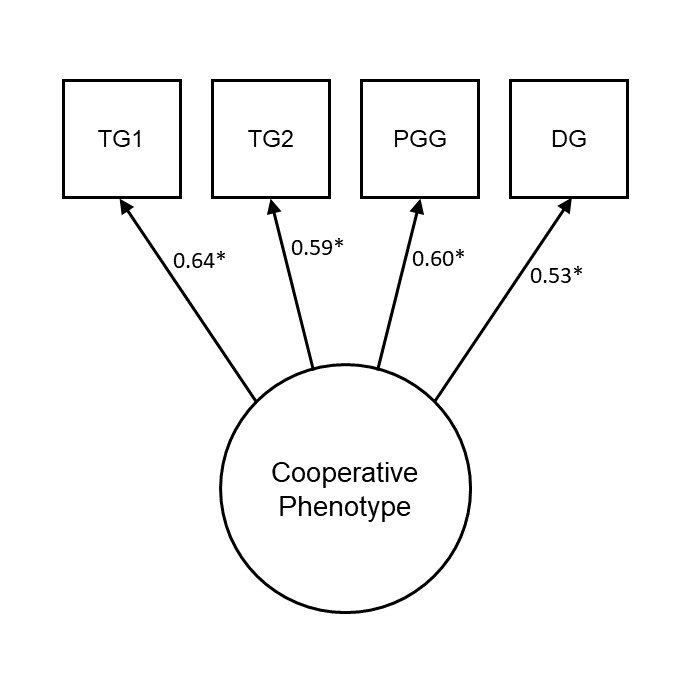
\includegraphics[width=0.8\linewidth]{images/cfa1} \caption{\emph{Confirmatory factor model for the cooperative
phenotype in Wave 2.} TG1 is treated as a binary endogenous variable. Numbers
are standardised coefficients. *\emph{p} \textless{} 0.05. TG1 = Trust Game (Give), TG2 = Trust
Game (Return), PGG = Public Goods Game, DG = Dictator Game.}\label{fig:cfa1Plot}
\end{figure}

\newpage





\begin{figure}
\centering
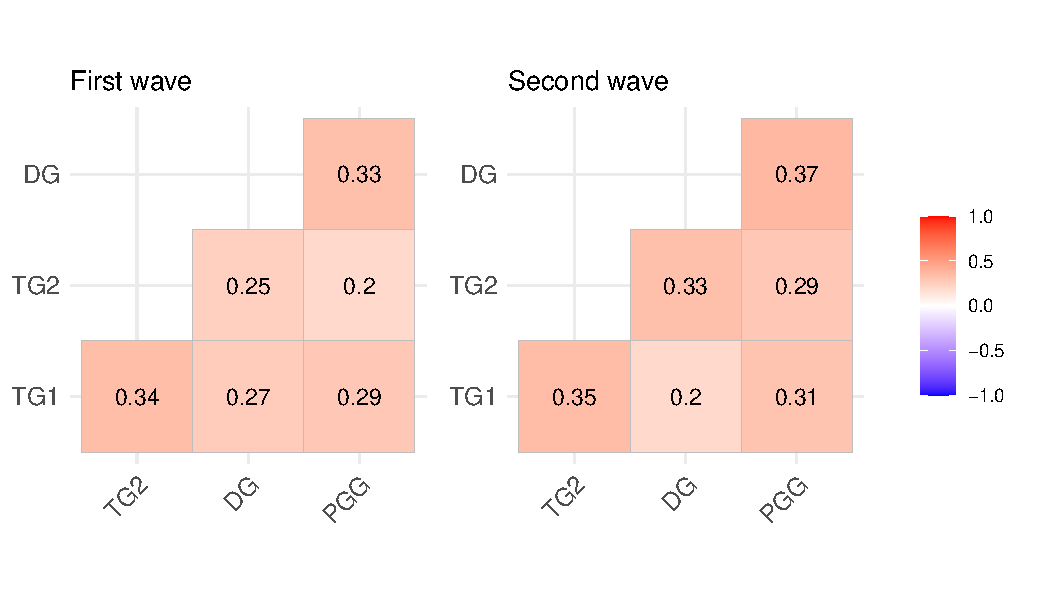
\includegraphics{manuscript_files/figure-latex/plotCors-1.pdf}
\caption{\label{fig:plotCors}\emph{Zero-order correlations between game decisions in the
first and second wave.} All \emph{p}-values \textless{} 0.01. TG1 = Trust Game (Give), TG2 =
Trust Game (Return), DG = Dictator Game, PGG = Public Goods Game.}
\end{figure}

\newpage





\begin{figure}
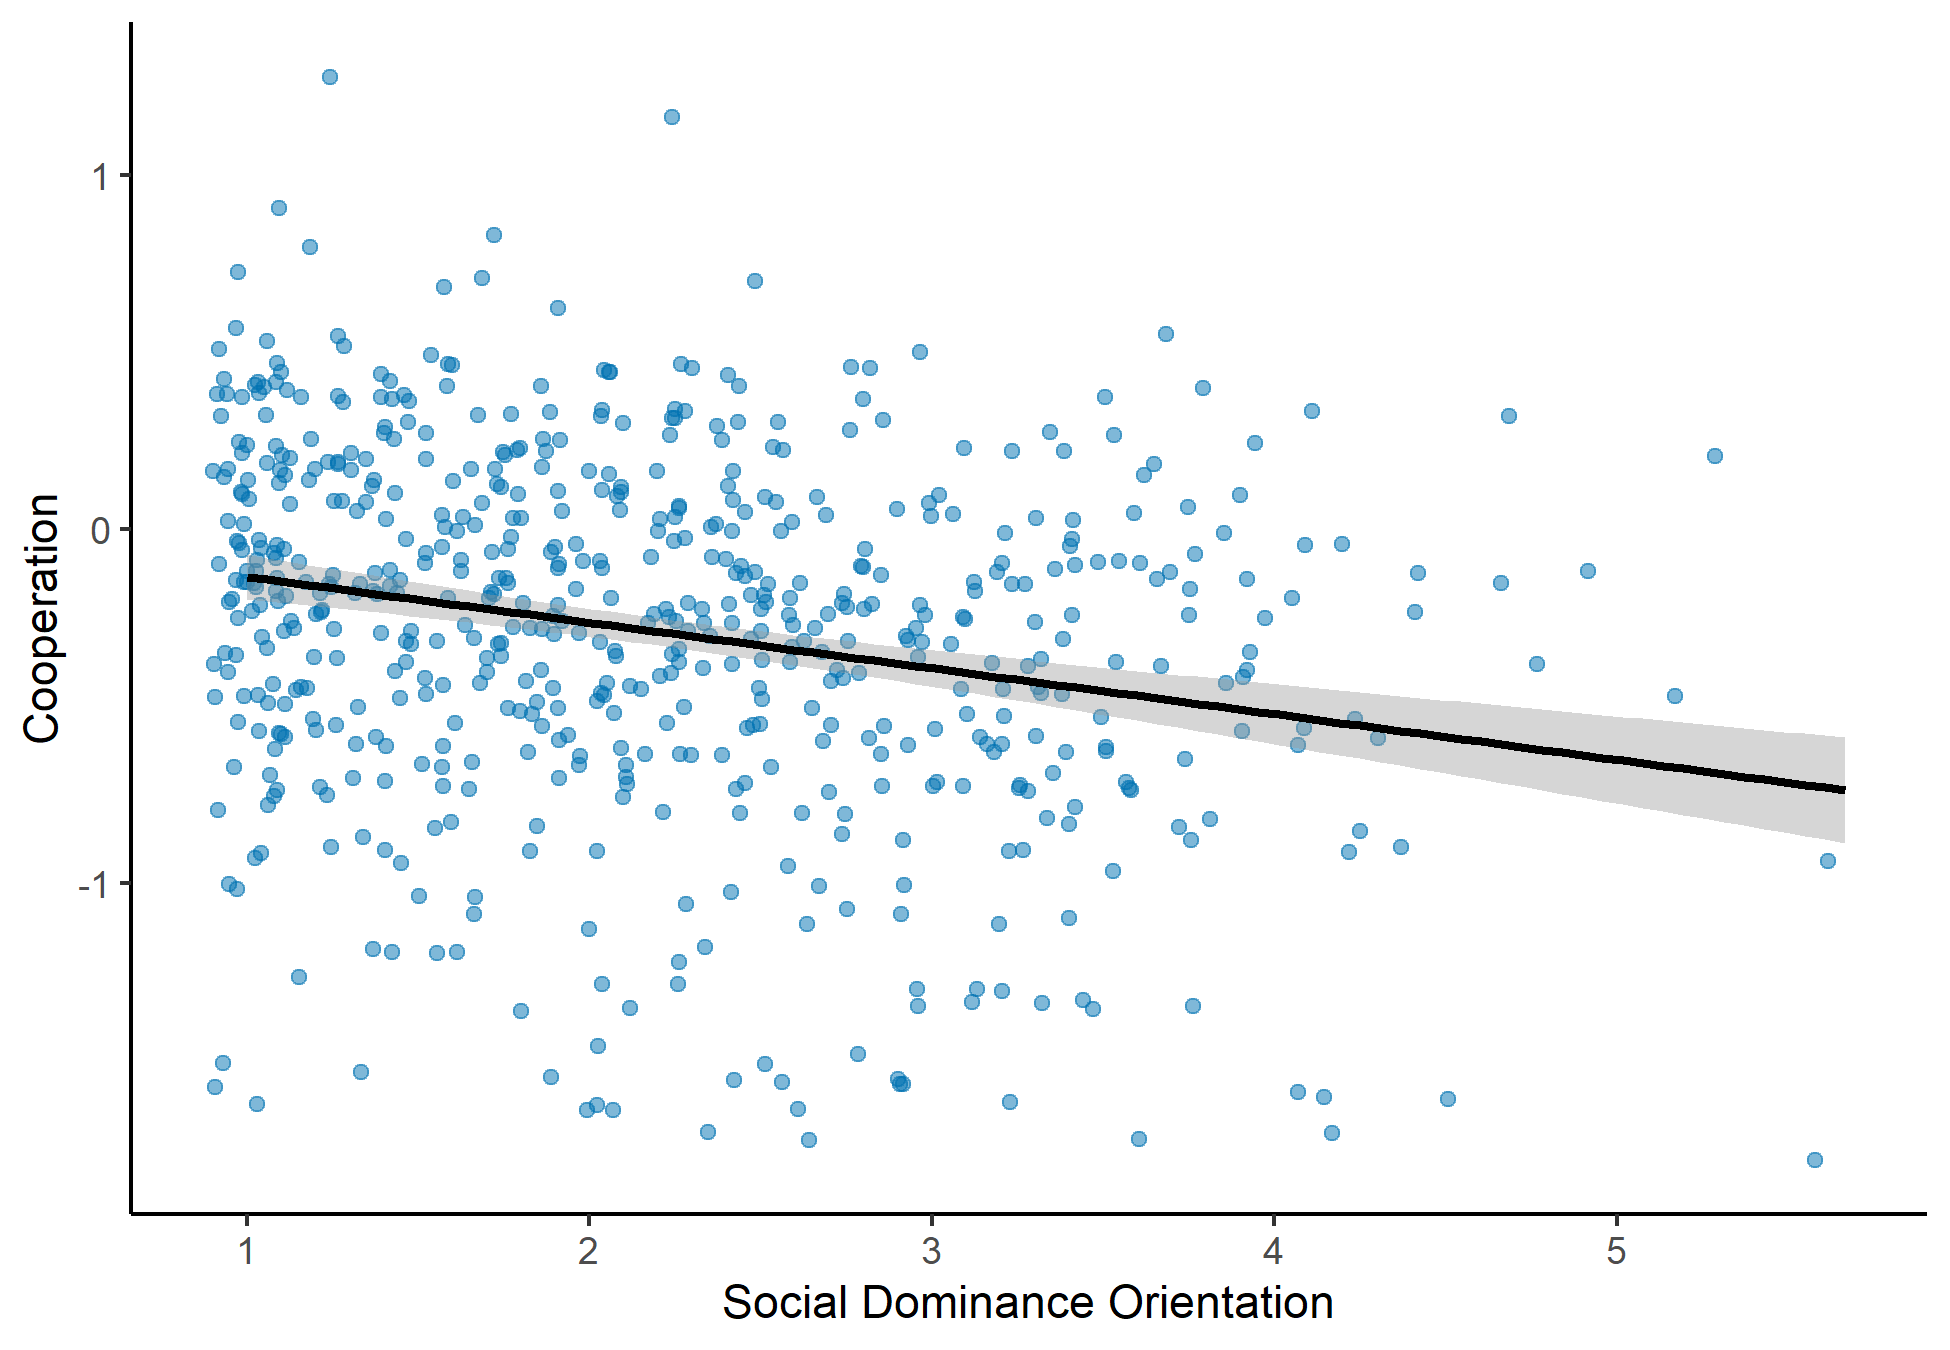
\includegraphics[width=0.8\linewidth]{manuscript_files/figure-latex/sem1Plot-1} \caption{\emph{Social Dominance Orientation (mean score) is
negatively related to model-predicted cooperation latent variable scores in the
second wave.}}\label{fig:sem1Plot}
\end{figure}

\newpage











\begin{figure}
\centering
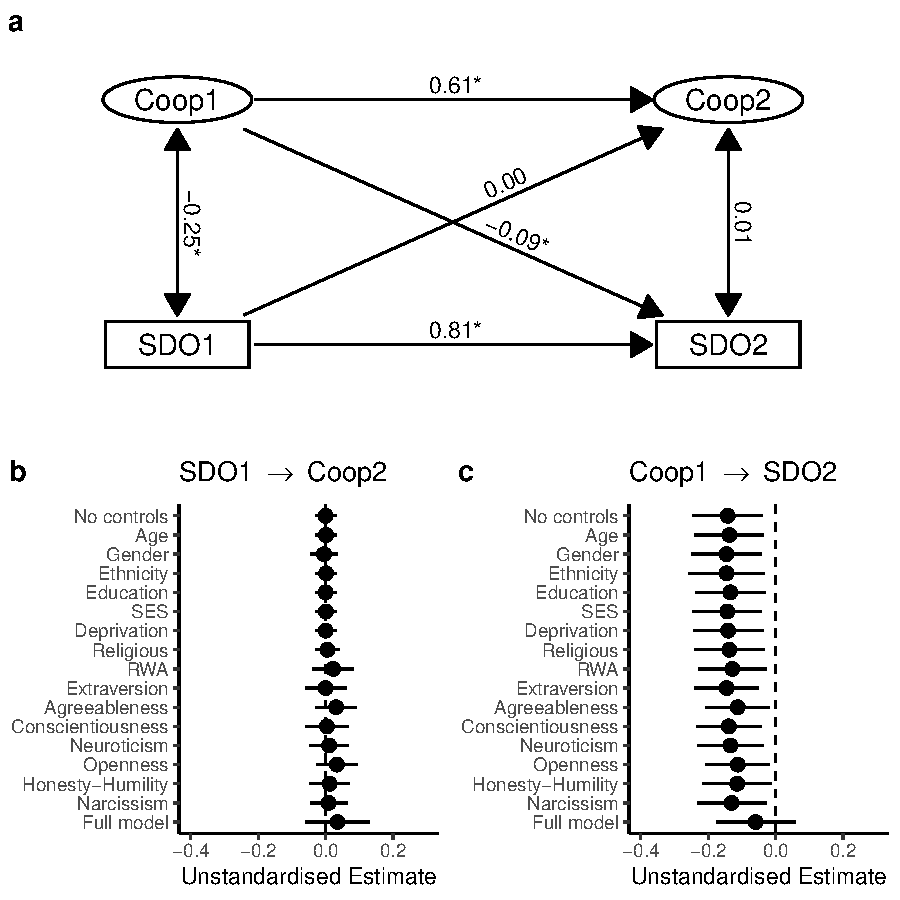
\includegraphics{manuscript_files/figure-latex/clpmPlotBSDO-1.pdf}
\caption{\label{fig:clpmPlotBSDO}\emph{Results of cross-lagged panel model with the
cooperative phenotype and SDO, analysing listwise-deleted data.} (a)
Autoregressive effects, cross-lagged effects, and within-wave (residual)
correlations from the model. Note that measurement models for the cooperative
phenotype latent variables are omitted from this figure. Numbers are
standardised coefficients, *\emph{p} \textless{} 0.05. (b, c) Forest plots visualising the
change in cross-lagged paths when controlling for time-invariant covariates,
individually and in a full model. Points are unstandardised estimates, lines
are 95\% confidence intervals.}
\end{figure}

\newpage












\begin{figure}
\centering
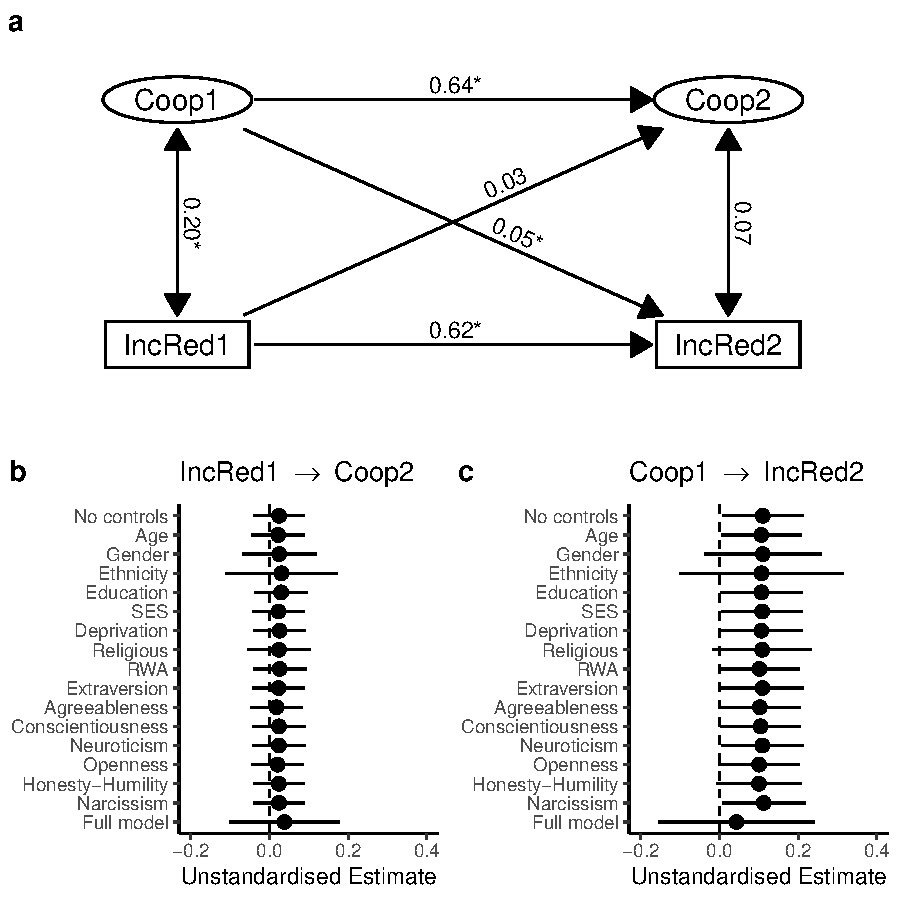
\includegraphics{manuscript_files/figure-latex/clpmPlotAIncRed-1.pdf}
\caption{\label{fig:clpmPlotAIncRed}\emph{Results of cross-lagged panel model with the
cooperative phenotype and support for income redistribution, pooling over 20
imputed datasets.} (a) Autoregressive effects, cross-lagged effects, and
within-wave (residual) correlations from the model. Support for income
redistribution is treated as ordinal. Note that measurement models for the
cooperative phenotype latent variables are omitted from this figure. Numbers are
standardised coefficients, *\emph{p} \textless{} 0.05. (b, c) Forest plots visualising the
change in cross-lagged paths when controlling for time-invariant covariates,
individually and in a full model. Points are unstandardised estimates, lines are
95\% confidence intervals.}
\end{figure}

\newpage












\begin{figure}
\centering
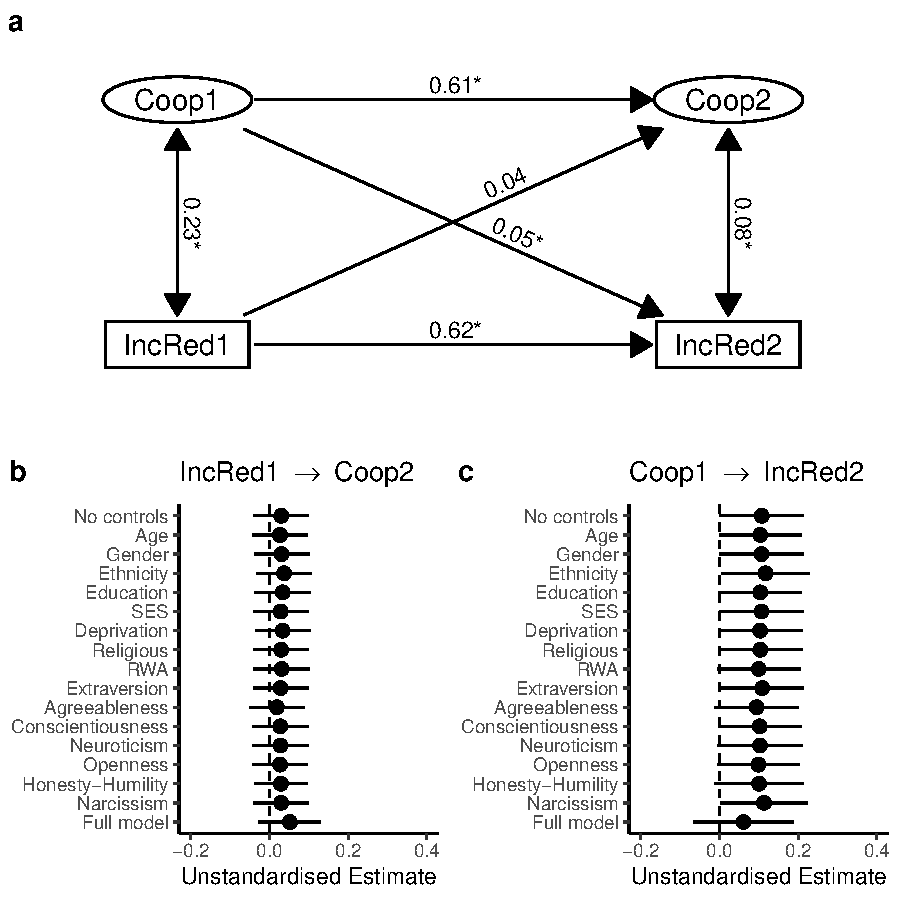
\includegraphics{manuscript_files/figure-latex/clpmPlotBIncRed-1.pdf}
\caption{\label{fig:clpmPlotBIncRed}\emph{Results of cross-lagged panel model with the
cooperative phenotype and support for income redistribution, analysing
listwise-deleted data.} (a) Autoregressive effects, cross-lagged effects, and
within-wave (residual) correlations from the model. Support for income
redistribution is treated as ordinal. Note that measurement models for the
cooperative phenotype latent variables are omitted from this figure. Numbers are
standardised coefficients, *\emph{p} \textless{} 0.05. (b, c) Forest plots visualising the
change in cross-lagged paths when controlling for time-invariant covariates,
individually and in a full model. Points are unstandardised estimates, lines are
95\% confidence intervals.}
\end{figure}

\newpage











\begin{figure}
\centering
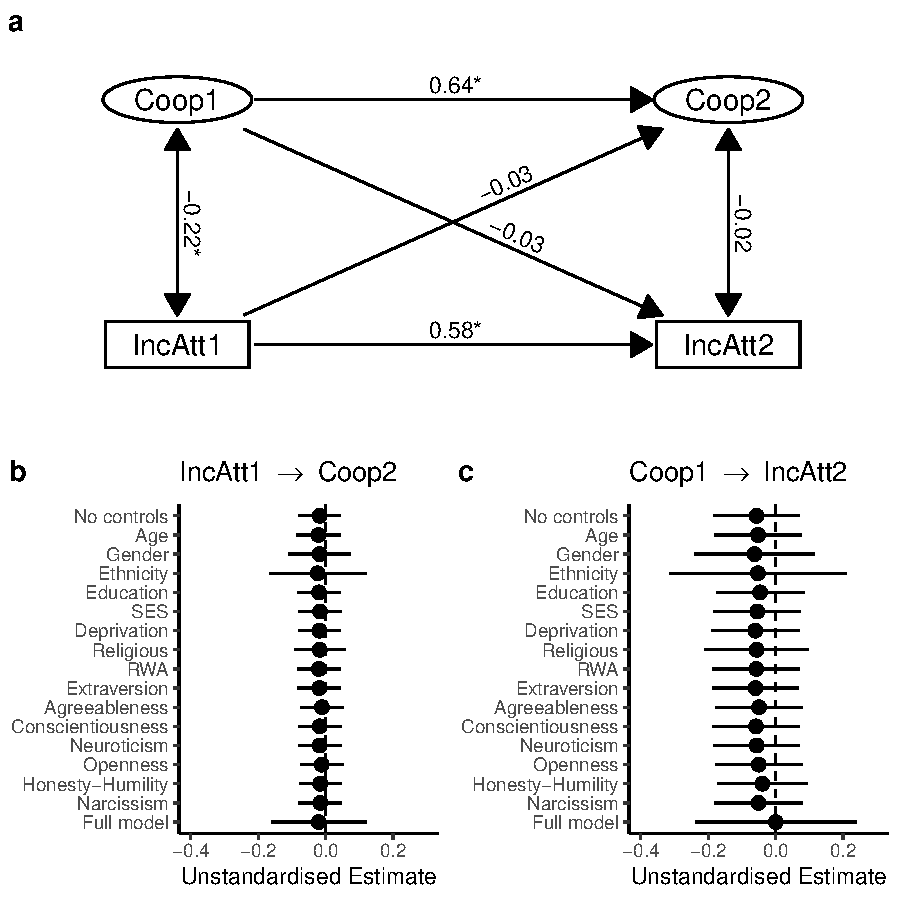
\includegraphics{manuscript_files/figure-latex/clpmPlotAIncAtt-1.pdf}
\caption{\label{fig:clpmPlotAIncAtt}\emph{Results of cross-lagged panel model with the
cooperative phenotype and income attribution beliefs, pooling over 20 imputed
datasets.} (a) Autoregressive effects, cross-lagged effects, and within-wave
(residual) correlations from the model. Income attribution beliefs are treated
as ordinal. Note that measurement models for the cooperative phenotype latent
variables are omitted from this figure. Numbers are standardised coefficients,
*\emph{p} \textless{} 0.05. (b, c) Forest plots visualising the change in cross-lagged paths
when controlling for time-invariant covariates, individually and in a full
model. Points are unstandardised estimates, lines are 95\% confidence intervals.}
\end{figure}

\newpage











\begin{figure}
\centering
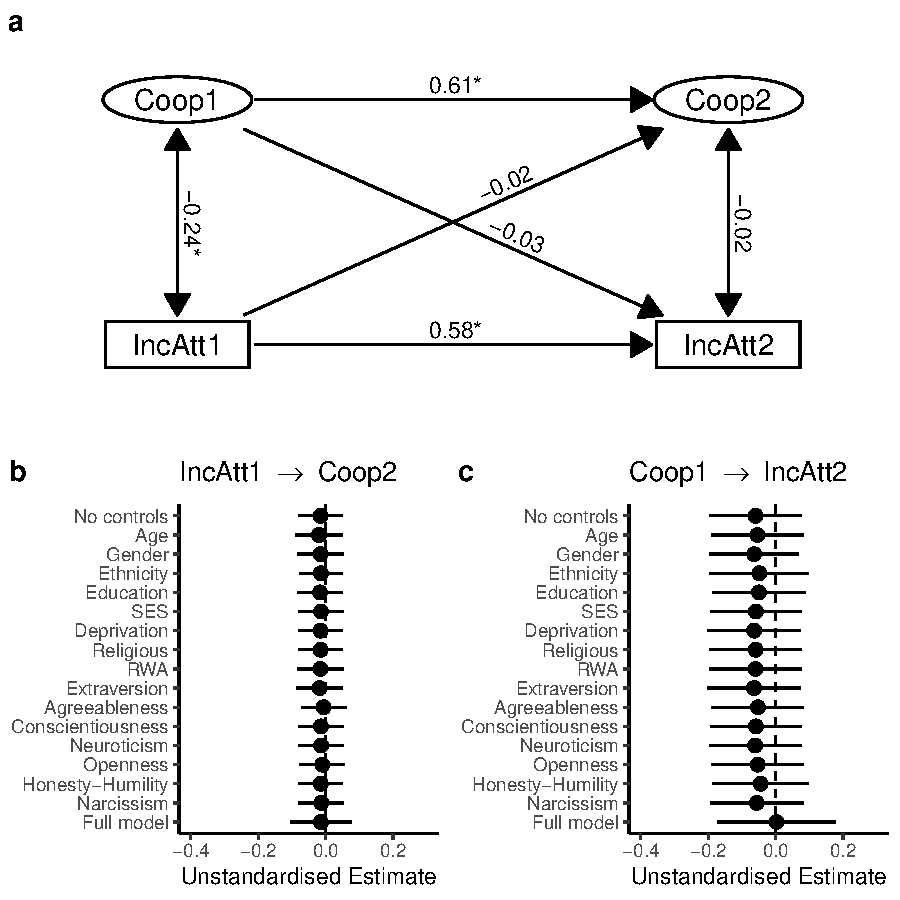
\includegraphics{manuscript_files/figure-latex/clpmPlotBIncAtt-1.pdf}
\caption{\label{fig:clpmPlotBIncAtt}\emph{Results of cross-lagged panel model with the
cooperative phenotype and income attribution beliefs, analysing listwise-deleted
data.} (a) Autoregressive effects, cross-lagged effects, and within-wave
(residual) correlations from the model. Income attribution beliefs are treated
as ordinal. Note that measurement models for the cooperative phenotype latent
variables are omitted from this figure. Numbers are standardised coefficients,
*\emph{p} \textless{} 0.05. (b, c) Forest plots visualising the change in cross-lagged paths
when controlling for time-invariant covariates, individually and in a full
model. Points are unstandardised estimates, lines are 95\% confidence intervals.}
\end{figure}

\newpage












\begin{figure}
\centering
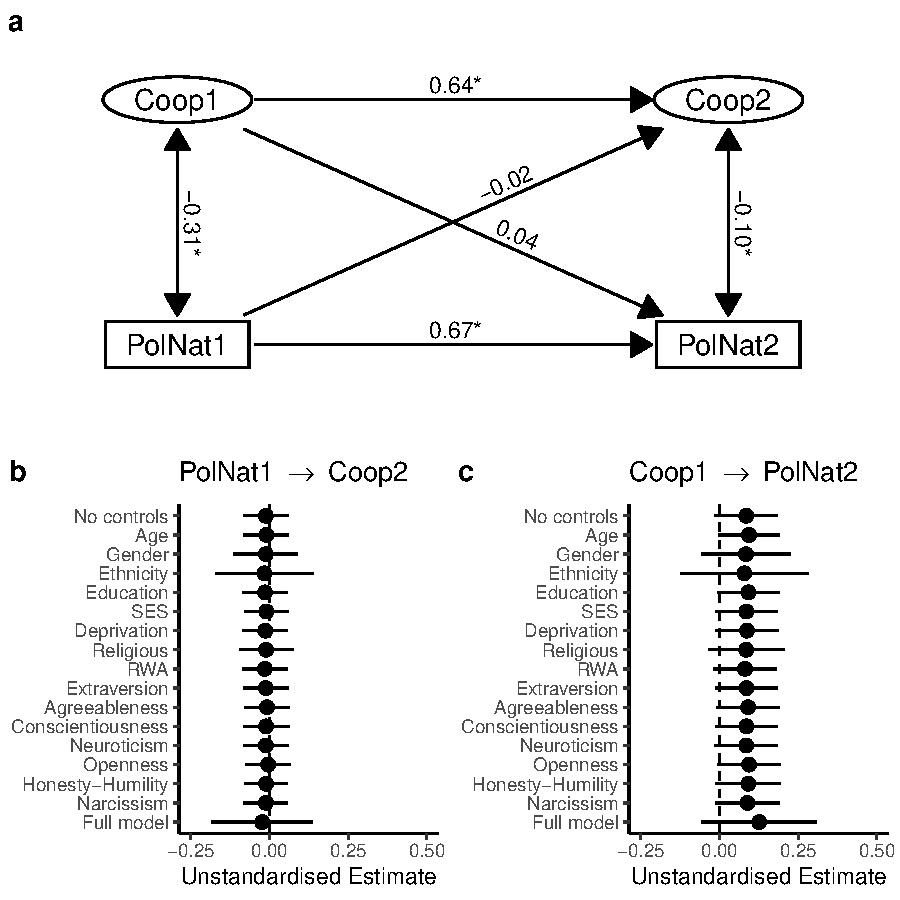
\includegraphics{manuscript_files/figure-latex/clpmPlotAPolNat-1.pdf}
\caption{\label{fig:clpmPlotAPolNat}\emph{Results of cross-lagged panel model with the
cooperative phenotype and support for the National Party, pooling over 20
imputed datasets.} (a) Autoregressive effects, cross-lagged effects, and
within-wave (residual) correlations from the model. Support for the National
Party is treated as ordinal. Note that measurement models for the cooperative
phenotype latent variables are omitted from this figure. Numbers are
standardised coefficients, *\emph{p} \textless{} 0.05. (b, c) Forest plots visualising the
change in cross-lagged paths when controlling for time-invariant covariates,
individually and in a full model. Points are unstandardised estimates, lines are
95\% confidence intervals.}
\end{figure}

\newpage












\begin{figure}
\centering
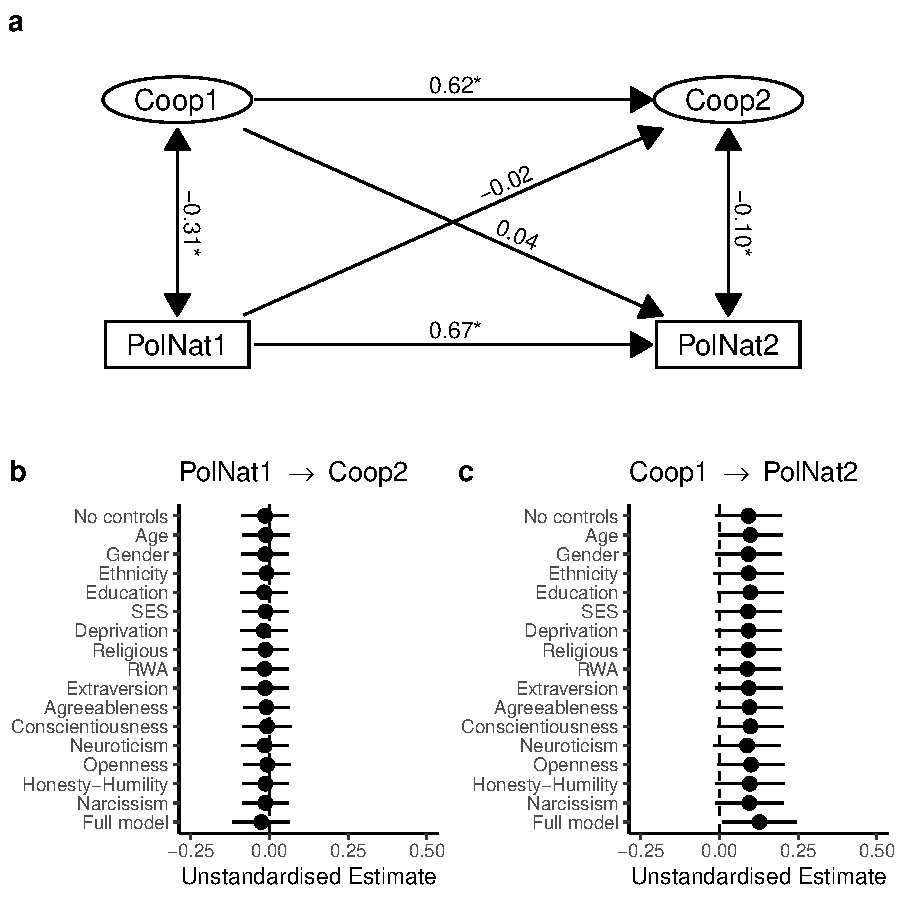
\includegraphics{manuscript_files/figure-latex/clpmPlotBPolNat-1.pdf}
\caption{\label{fig:clpmPlotBPolNat}\emph{Results of cross-lagged panel model with the
cooperative phenotype and support for the National Party, analysing
listwise-deleted data.} (a) Autoregressive effects, cross-lagged effects, and
within-wave (residual) correlations from the model. Support for the National
Party is treated as ordinal. Note that measurement models for the cooperative
phenotype latent variables are omitted from this figure. Numbers are
standardised coefficients, *\emph{p} \textless{} 0.05. (b, c) Forest plots visualising the
change in cross-lagged paths when controlling for time-invariant covariates,
individually and in a full model. Points are unstandardised estimates, lines are
95\% confidence intervals.}
\end{figure}

\newpage

\hypertarget{supplementary-tables}{%
\subsection{Supplementary Tables}\label{supplementary-tables}}







\begin{table}[H]

\begin{center}
\begin{threeparttable}

\caption{\label{tab:biasTable}Results of linear models estimating the differences in
key variables between participants who dropped out (n = 414) and participants
who completed both waves of data collection (n = 631). All models show no
significant differences between dropouts and non-dropouts, suggesting that our
sample was not systematically biased by retention.}

\begin{tabular}{lllll}
\toprule
Variable & \multicolumn{1}{c}{b} & \multicolumn{1}{c}{SE} & \multicolumn{1}{c}{t} & \multicolumn{1}{c}{p}\\
\midrule
egame.TG1.T10 & 0.00 & 0.03 & -0.05 & 0.96\\
egame.TG2.T10 & -1.11 & 1.83 & -0.61 & 0.55\\
egame.PGG.T10 & 1.43 & 1.99 & 0.72 & 0.47\\
egame.DG.T10 & -0.31 & 1.26 & -0.25 & 0.80\\
T10.SDO & 0.05 & 0.06 & 0.86 & 0.39\\
Issue.IncomeRedistribution.T10 & 0.03 & 0.12 & 0.28 & 0.78\\
IncomeAttribution.T10 & 0.04 & 0.12 & 0.38 & 0.70\\
Pol.SupNational.T10 & 0.15 & 0.13 & 1.20 & 0.23\\
\bottomrule
\end{tabular}

\end{threeparttable}
\end{center}

\end{table}

\newpage




\begin{lltable}

\footnotesize{

\begin{longtable}{p{5cm}p{14cm}p{1cm}}\noalign{\getlongtablewidth\global\LTcapwidth=\longtablewidth}
\caption{\label{tab:itemTable}Self-report items from the New Zealand Attitudes and
Values Study.}\\
\toprule
Item & \multicolumn{1}{c}{Description / Text} & \multicolumn{1}{c}{Wave}\\
\midrule
\endfirsthead
\caption*{\normalfont{Table \ref{tab:itemTable} continued}}\\
\toprule
Item & \multicolumn{1}{c}{Description / Text} & \multicolumn{1}{c}{Wave}\\
\midrule
\endhead
SDO1 & It is OK if some groups have more of a chance in life than others & 10 - 11\\
SDO2 & Inferior groups should stay in their place & 10 - 11\\
SDO3 & To get ahead in life, it is sometimes okay to step on other groups & 10 - 11\\
SDO4 (reversed) & We should have increased social equality & 10 - 11\\
SDO5 (reversed) & It would be good if groups could be equal & 10 - 11\\
SDO6 (reversed) & We should do what we can to equalise conditions for different groups & 10 - 11\\
RWA1 & It is always better to trust the judgment of the proper authorities in government and religion than to listen to the noisy rabble-rousers in our society who are trying to create doubt in people's minds & 10\\
RWA2 & It would be best for everyone if the proper authorities censored magazines so that people could not get their hands on trashy and disgusting material & 10\\
RWA3 & Our country will be destroyed some day if we do not smash the perversions eating away at our moral fibre and traditional beliefs & 10\\
RWA4 (reversed) & People should pay less attention to The Bible and other old traditional forms of religious guidance, and instead develop their own personal standards of what is moral and immoral & 10\\
RWA5 (reversed) & Atheists and others who have rebelled against established religions are no doubt every bit as good and virtuous as those who attend church regularly & 10\\
RWA6 (reversed) & Some of the best people in our country are those who are challenging our government, criticizing religion, and ignoring the 'normal way' things are supposed to be done & 10\\
Income redistribution & Redistributing money and wealth more evenly among a larger percentage of the people in New Zealand through heavy taxes on the rich & 10 - 11\\
Income attribution & If incomes were more equal, people would be less motivated to work hard & 10 - 11\\
Support for National Party & Level of support for The National Party & 10 - 11\\
Age & What is your date of birth? & 10\\
Gender & What is your gender? (open-ended) & 10\\
Ethnicity & Which ethnic group do you belong to? (NZ census question) & 10\\
Education level & NZ Reg (0-10 education ordinal rank) & 10\\
Socio-economic status & NZSEI13 (NZ Socio-economic index) & 10\\
Local deprivation & Deprivation score 2013 (for Meshblock) & 10\\
Religiosity & Do you identify with a religion and/or spiritual group? & 10\\
Extraversion1 & Am the life of the party & 10\\
Extraversion2 (reversed) & Don't talk a lot & 10\\
Extraversion3 (reversed) & Keep in the background & 10\\
Extraversion4 & Talk to a lot of different people at parties & 10\\
Agreeableness1 & Sympathize with others' feelings & 10\\
Agreeableness2 (reversed) & Am not interested in other people's problems & 10\\
Agreeableness3 & Feel others' emotions & 10\\
Agreeableness4 (reversed) & Am not really interested in others & 10\\
Conscientiousness1 & Get chores done right away & 10\\
Conscientiousness2 & Like order & 10\\
Conscientiousness3 (reversed) & Make a mess of things & 10\\
Conscientiousness4 (reversed) & Often forget to put things back in their proper place & 10\\
Neuroticism1 & Have frequent mood swings & 10\\
Neuroticism2 (reversed) & Am relaxed most of the time & 10\\
Neuroticism3 & Get upset easily & 10\\
Neuroticism4 (reversed) & Seldom feel blue & 10\\
Openness1 & Have a vivid imagination & 10\\
Openness2 (reversed) & Have difficulty understanding abstract ideas & 10\\
Openness3 (reversed) & Do not have a good imagination & 10\\
Openness4 (reversed) & Am not interested in abstract ideas & 10\\
Narcissism1 & Feel entitled to more of everything & 10\\
Narcissism2 & Deserve more things in life & 10\\
Honesty-Humility1 (reversed) & Would like to be seen driving around in a very expensive car & 10\\
Honesty-Humility2 (reversed & Would get a lot of pleasure from owning expensive lucury goods & 10\\
\bottomrule
\end{longtable}

}

\end{lltable}

\newpage







\begin{table}[H]

\begin{center}
\begin{threeparttable}

\caption{\label{tab:diffTable}Results of multilevel models estimating the differences
in game behaviour between the two waves. There are no significant differences
between waves for the Trust Game and the Public Goods Game. In the Dictator
Game, participants give 2 fewer points (out of 100) in the second wave, on
average.}

\begin{tabular}{lllll}
\toprule
Game & \multicolumn{1}{c}{b} & \multicolumn{1}{c}{SE} & \multicolumn{1}{c}{t} & \multicolumn{1}{c}{p}\\
\midrule
Trust Game (Give) & 0.02 & 0.02 & 0.72 & 0.47\\
Trust Game (Return) & 0.00 & 0.01 & -0.42 & 0.67\\
Public Goods Game & 0.02 & 0.01 & 1.28 & 0.20\\
Dictator Game & -0.02 & 0.01 & -2.35 & 0.02\\
\bottomrule
\end{tabular}

\end{threeparttable}
\end{center}

\end{table}

\newpage






\begin{table}[H]

\begin{center}
\begin{threeparttable}

\caption{\label{tab:tableCompareMI}\emph{Measurement invariance analysis of the cooperative
phenotype latent variable supports strict measurement invariance.} CFI =
Comparative Fit Index; RMSEA = Root Mean Square Error of Approximation; SRMR =
Standardised Root Mean Square Residual.}

\begin{tabular}{lllllllll}
\toprule
Model & \multicolumn{1}{c}{$\chi^2$} & \multicolumn{1}{c}{df} & \multicolumn{1}{c}{CFI} & \multicolumn{1}{c}{RMSEA} & \multicolumn{1}{c}{SRMR} & \multicolumn{1}{c}{$\Delta$CFI} & \multicolumn{1}{c}{$\Delta$RMSEA} & \multicolumn{1}{c}{$\Delta$SRMR}\\
\midrule
Configural & 26.70 & 15 & 0.991 & 0.035 & 0.038 & - & - & -\\
Metric & 37.61 & 18 & 0.985 & 0.042 & 0.044 & -0.006 & 0.006 & 0.005\\
Scalar & 41.90 & 22 & 0.985 & 0.038 & 0.044 & 0.000 & -0.004 & 0.000\\
Strict & 44.87 & 25 & 0.985 & 0.036 & 0.044 & 0.000 & -0.002 & 0.001\\
\bottomrule
\end{tabular}

\end{threeparttable}
\end{center}

\end{table}


\end{document}
